%% this chapter sets up the foundational system, which is Univalent Foundations
\label{ch:univalent-mathematics}

\section{What is a type?}
\label{sec:what-is-a-type}

In some computer programming languages, all variables are introduced along with a declaration of the type of thing they will refer to.  For example,
one may encounter types such as $bool$, $string$, $int$, and $real$, describing Boolean values, character strings, 32 bit integers, and 64 bit
floating point numbers.  The types are used to determine which statements of the programming language are grammatically well-formed.
For example, if $s$ of type $string$ and $x$ is of type $real$, we may write $1/x$, but we may not write $1/s$.

Types occur in mathematics, too, and are used in the same way: all variables are introduced along with a declaration of the type of thing they
will refer to.  For example, one may say ``consider a point $P$ of the plane'', ``consider a line $L$ of the plane'', ``consider a hexagon
$H$'', or ``consider a graph $G$''.  The types are used to determine which mathematical statements are grammatically well-formed.  For example,
one may write ``$P$ lies on $L$'' or ``$L$ passes through $P$'', but not ``$L$ lies on $P$''.

In \emph{univalent mathematics}, types are used to classify all mathematical objects.  Every mathematical object is an element of some (unique)
type.

One expresses the statement that an ``element'' $a$ is of ``type'' $X$ by writing $a:X$.  Using that notation, each variable is introduced along
with a declaration of the type of thing it will refer to, and the declared types of the variables are used to determine which statements of the
theory are grammatically well-formed.

There are enough ways to form new types from old ones to provide everything we need to write mathematics.

If $X$ and $Y$ are types, there will be a type whose elements serve as 
\emph{functions} from $X$ to $Y$; the notation for it is $X \to Y$.  
Thus when we write $f : X \to Y$, we mean that $f$ is an element of the type $X \to Y$, 
and we are saying that $f$ is a function from $X$ to $Y$.

Functions behave as one would expect, and one can make new ones in the usual way.

To provide an example of making new functions in the usual way, we first introduce notation for making and for using {\em definitions}.  The
notation $x \defeq z$ will be an announcement that we are defining the expression $x$ to be the expression $z$; the forms allowed for the
expression $x$ will be made clear by the examples we give.  The notation $x \jdeq y$ will denote the statement that the expressions $x$ and $y$
become the same thing if all the subexpressions within $x$ or $y$ are expanded according to their definitions, if any; in that case, we will say
that $x$ and $y$ are \emph{the same by definition}.  Whenever two expressions are the same by definition, we may replace one with the other
inside any other expression, at will, because the expansion of definitions is regarded as trivial and transparent.

We proceed now to the promised example.  Consider functions $f : X \to Y$ and $g : Y \to Z$.  We define their composite $g \circ f : X \to Z$ by
setting $g \circ f \defeq (a \mapsto g(f(a)))$; in other words, it is the function that sends an arbitrary element $a$ of $X$ to $g(f(a))$ in
$Z$.  The composite $g \circ f$ may also be denoted simply by $gf$.

Now consider functions $f : X \to Y$, $g : Y \to Z$, and $h : Z \to W$.  Then $(h \circ g) \circ f$ and $h \circ (g \circ f)$ are the same by
definition, since applying the definitions within expands both expresssions to $a \mapsto h(g(f(a)))$.  In other
words, we have established that $(h \circ g) \circ f \jdeq h \circ (g \circ f)$.

One may define the identity function $id_X : X \to X$ by setting $id_X \defeq (a \mapsto a)$.  Application of definitions shows that $f \circ
id_X$ is the same by definition as $a \mapsto f(a)$, which, by a standard convention, which we adopt, is to be regarded as the same as $f$.  In
other words, we have established that $f \circ id_X \jdeq f$.  A similar computation applies to $id_Y \circ f$.

In the following sections we will expose various other elementary types and elementary ways to make new types from old ones.

\section{The type of natural numbers}
\label{sec:natural-numbers}

Here are Peano's rules \citep{peano-principia} for constructing the natural numbers in the form that is used in type theory.
\begin{enumerate}
\item[P1:] there is a type called $\NN$ (whose elements will be called natural numbers);
\item[P2:] there is an element of $\NN$ called $0$;
\item[P3:] if $m$ is a natural number, then there is also a natural number $S(m)$, called the \emph{successor} of $m$;
\item[P4:] given a family of types $X(m)$ depending on a parameter\footnote{
  Referring to a variable as a {\em parameter} is a turn of phrase that emphasizes that an expression depends on the variable,
  drawing attention to the results as the variable ranges over elements of its type.
  }
  $m$ of type $\NN$, in order to define a family $f(m) : X(m)$ of elements of each of them it suffices to provide an element $a$ of $X(0)$ and
  to provide, for each $m$, a function $g_m : X(m) \to X(S(m))$.  (The resulting function $f$ may be regarded as having been defined inductively
  by the two declarations $f(0) \defeq a$ and $f(S(m)) \defeq g_m(f(m))$.)
\end{enumerate}
\nopagebreak
You may recognize rule P4 as ``the principle of mathematical induction'' or as ``defining a function by recursion''.  We may also refer to it
simply as ``induction for $\NN$''.  Notice that the two cases in an inductive definition correspond to the two ways of introducing elements of
$\NN$ via the use of rules P2 and P3.

We introduce the following syntactic definitions.
\begin{align*}
 1 & \defeq S(0) \\
 2 & \defeq S(1) \\
 3 & \defeq S(2) \\
 \vdots
\end{align*}

We may now define addition and multiplication of natural numbers by recursion.  In both cases, the family of types $X(m)$ is defined by setting
$X(m) \defeq \NN$ for every $m : \NN$.  For natural numbers $n$ and $m$ we define $n+m : \NN$ by induction on $m$ by setting $n+0\defeq n$ and
$n+S(m)\defeq S(n+m)$.  Application of definitions shows, for example, that $2+2 \jdeq 4$ are the same by definition, because both sides reduce
to $S(S(S(S(0))))$.  Similarly we define the product $n \cdot m : \NN$ by induction on $m$ by setting setting $n\cdot 0\defeq 0$ and $n\cdot
S(m)\defeq (n\cdot m) + n$.

We may also define the factorial function $\fact : \NN \to \NN$ by recursion, setting $\fact(0) \defeq 1$ and setting
$\fact(S(m)) \defeq (m+1) \cdot \fact(m)$.  This definition applies rule P4 with $1$ for $a$, and with the
function $n \mapsto (m+1) \cdot n$ for $g_m$, for all $m$.
Application of the definitions shows, for example, that $\fact(2) \jdeq 2$, because both sides expand to $S(S(0))$.

We finish this section with the definition of iteration by recursion.  Let $X$ be a type, and suppose we have a function $e : X \to X$.  We
define by induction the $n$-fold \emph{iteration} $e^n : X \to X$ by setting $e^0 \defeq \id_X$ and $e^{S(n)}\defeq e\circ e^n$.
Here we apply rule P4 with the identity function $\id_X$ for $a$
and the function $d \mapsto e\circ d$ for $g_m : (X\to X)\to(X\to X)$, for any $m$.

\section{Identity types}
\label{sec:identity-types}

One of the most important types is the \emph{identity type}, which implements the intuitive notion of equality; the reader may be more
comfortable if we call it the \emph{equality type}, at least initially.  Identity (or equality) between two elements may be considered only when
the two elements are of the same type; we shall have no need to compare elements of different types.

Here are the rules for constructing equality types.
\begin{enumerate}
\item[E1:]
  for any type $X$ and for any elements $a$ and $b$ of it, there is a type $a =_X b$;
\item[E2:] for any type $X$ and for any element $a$ of it, there is an element $\refl a$ of type $a =_X a$ (the name $\refl{}$ comes from the word
  ``reflexivity'')
\item[E3:] for any type $X$ and for any element $a$ of it, given a family of types $P(b,e)$ depending on parameters $b$ of type $X$ and $e$ of type
  $a =_X b$, in order to define elements $f(b,e) : P(b,e)$ of all of them it suffices to provide an element $p$ of $P(a,\refl a)$.  The resulting
  function $f$ may be regarded as having been completely defined by the single definition $f(a,\refl a) \defeq p$.
\end{enumerate}

The identity type $a =_X b$ may also be called an {\em equation}.

When there is no risk of confusion, we will write $a=b$ instead of $a =_X b$.

When we know that there can be at most one element of $a=b$, we will refer to an element $i$ of $a=b$ as a {\em proof}\,\footnote{Here we override
  the use of the word ``proof'' that is traditional in metamathematics; such a thing would now be a formal expression denoting an
  element of $a=b$.} that $a$ is equal to $b$.

When $a=b$ may have more than one element, we will refer to an element $i$ of $a=b$ as an {\em identification} of $a$ with $b$, or simply as an
{\em identity} or an {\em equality}.  Since the word ``identification'' is a long one, we may also refer to $i$ as a {\em path} from $a$ to
$b$---this has the advantage of incorporating the intuition that an identification may proceed gradually through intermediate steps.

It may come as a surprise that two mathematical objects can be equal in more than one way, especialy since rule E3 above seems to say that the
trivial proofs of equality are the only relevant ones, but this reflects a situation commonly encountered in geometry, where {\em congruence} of
geometric figures is considered.  For example, in Euclidean space, two equilateral triangles of the same size are congruent in six (different)
ways.  The chief novelty of univalent mathematics is that the basic logical notion of equality, as implemented by the types $a=b$, is carefully
engineered to accommodate notions of congruence and symmetry from diverse areas of mathematics, including geometry.  Exposing that point of view
in the context of geometry is the main point of this book.

In light of the analogy with geometry just introduced, we will refer to an element $i$ of $a=a$ as a {\em symmetry} of $a$.  Think of a
congruence of a triangle with itself.  An example of a non-trivial symmetry will be seen in \cref{xca:C2}.

Expansion of the definitions in the type $\fact(2)=2$ simplifies it to $S(S(0)) = S(S(0))$, so we see from rule E2 that $\refl{S(S(0))}$ serves
as a proof of it.  We may also write $\refl{2}$ and $\refl{\fact(2)}$ for that proof.  A student might want a more detailed proof of the
equation, but as a result of our convention above that definitions are syntactically transparent, the application of definitions, including
inductive definitions, is regarded as a trivial operation, and the details are omitted from the proof.

We will refer to rule E3 as ``induction for equality''.  It says that to prove something about (or to construct something from) every proof that
$a$ is equal to something else, it suffices to consider the special case where the proof is the trivial proof that $a$ is equal to itself, i.e.,
where the proof is $\refl a : a=a$.  Notice that the single case in such an induction corresponds to the single way of introducing elements of
equality types via rule E2, and compare that with P4, which dealt with the two ways of introducing elements of $\NN$.
%% ???
Intuitively, the induction principle for equality amounts to saying that the element $\refl a$ ``generates'' the system of types $a=b$, as $b$
ranges over elements of $A$.

Equality is {\em symmetric}, in the sense that an identification of $a$ with $b$ may be reversed to give an identification of $b$ with $a$.  In
order to produce an element of $b=a$ from an element $p$ of $a=b$, for any $b$ and $p$, we argue by induction.  We let $P(b,e)$ be $b=a$ for any
$b$ of type $X$ and for any $e$ of type $a=b$, for use in rule E3 above. 
This reduces us to the case where $b$ is $a$ and $p$ is $\refl a$, and
our task is now to produce an element of $a=a$; we choose $\refl a$ for it.

Equality is also {\em transitive}, and is established the same way.  
For each $a,b,c:X$ and for each $p:a=b$ and for each $q:b=c$ we want to produce an
element of type $a=c$.  By induction on $q$ we are reduced to the case where $c$ is $b$ and $q$ is $\refl b$, and we are to produce an element
of $a=b$.  The element $p$ serves the purpose.  
%Notice the similarity of this inductive definition with the definition given above 
%of the sum $m+n$. HMM ... (left versus right recursion)

Now we state our symmetry result a little more formally.

\begin{definition}\label{def:eq-symm}
For any type $X$ and for any $a,b:X$, let $\symm_{a,b} : (a=b) \to (b=a)$ 
be the function defined by induction by setting
$\symm_{a,a}(\refl a) \defeq \refl a$.
We may abbreviate $\symm_{a,b}(p)$ as $p^{-1}$.
\end{definition}

Similarly, transitivity is formulated as an inductive definition for 
a function $\trans_{a,b,c} : (a=b) \to ((b=c) \to (a=c))$.  We may
abbreviate $(\trans_{a,b,c}(p))(q)$ as either $p\ct q$, 
or as $q\cdot p$, $qp$, or $q\circ p$, see \cref{fig:path-concatenation}.
(The notation $q\circ p$ will be used when $a,b,c$ are types and
$p$ and $q$ come from equivalences $a\to b$ and $b\to c$, respectively.)


\begin{figure}
  \centering
  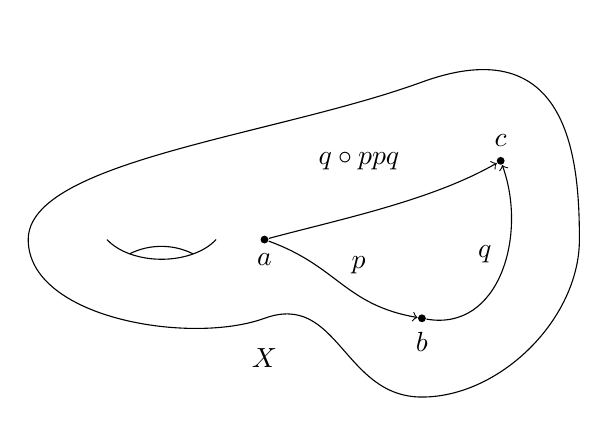
\begin{tikzpicture}
    \node (X) at (0,-1.5) {$X$};
    \draw (0,-1)
    .. controls ++(200:-1) and ++(180:1) .. (2,-2)
    .. controls ++(180:-1) and ++(270:1) .. (4,0)
    .. controls ++(270:-1) and ++(20:2)   .. (2,2)
    .. controls ++(20:-2)   and ++(90:1)  .. (-3,0)
    .. controls ++(90:-1)  and ++(200:1) .. (0,-1);
    \node[fill,circle,inner sep=1pt,label=below:$a$] (a) at (0,0) {};
    \node[fill,circle,inner sep=1pt,label=below:$b$] (b) at (2,-1) {};
    \node[fill,circle,inner sep=1pt,label=above:$c$] (c) at (3,1) {};
    \node (ct) at (1.2,1) {$q\circ p \jdeq p\ct q$};
    \draw[->] (a) .. controls ++(-20:1) and ++(170:1) .. node[auto] {$p$} (b);
    \draw[->] (b) .. controls ++(170:-1) and ++(-70:1) .. node[auto] {$q$} (c);
    \draw[->] (a) .. controls ++(15:1) and ++(210:1) .. (c);
    \draw (-2,0) arc(210:330:.8 and .5);
    \draw (-0.91,-.18) arc(60:120:.8 and .7);
  \end{tikzpicture}
  
  \caption{Concatenation of paths in $X$}
  \label{fig:path-concatenation}
\end{figure}

The types of $\symm_{a,b}$ and $\trans_{a,b,c}$ express that
equality is symmetric and transitive. Another view on
$\symm_{a,b}$ and $\trans_{a,b,c}$ is that they are
operations on identifications, namely reversing an identification
and concatenating two identifications. As operations, they satisfy
many algebraic properties, such as $(p^{-1})^{-1} = p$ and
associativity of concatenation, that are all easy to prove by induction. 
We leave them as exercises, see \cite[Lemma 2.1.4]{hottbook}. 

Concatenation can be used to define powers $p^n$ of $p:a=a$
by induction on $n:\NN$, setting $p^0\defeq\refl{a}$ and
$p^{n+1}\defeq p\cdot p^n$. Negative powers $p^{-n}$ are defined
as $(p^{-1})^n$.

One frequent use of elements of identity types is in \emph{substitution}.  
Let $X$ be a type, and let $T(x)$ be a family of types depending on a
parameter $x:X$.  Suppose $x,y:X$ and $e:x=y$.  
Then there is a function of type $T(x) \to T(y)$. 
We define one specific such function by induction, 
by taking its value to be the identity function on $T(x)$ 
in the case of $\refl{x}:x=x$.

\begin{definition}\label{def:transport} The function
  \[ 
  \trp{T,e} : T(x) \to T(y)
  \]
  is defined by induction setting $\trp{T,\refl{x}} (t) \defeq t$.
\end{definition} 
The function thus defined may be called 
\emph{the transport function in the type family $T$ along the path $e$}, 
 or, less verbosely, \emph{transport}.
 We may also simplify the notation to just $\trp e$.
The transport functions behave as expected: transport along the composition
$e\cdot e'$ is the composition of the two transport functions (to be
 proved by induction).

When the types $T(x)$ may have more than one element, 
we may regard an element of $T(x)$ as providing additional {\em structure} on $x$. 
In that case, we will refer to the transport function $T(x) \to T(y)$ as 
\emph{transport of structure} from $x$ to $y$. 

Take, for example, $T(x)\defeq (x=x)$. 
Then $\trp e$ is of type $x=x \to y=y$ and transports the
symmetries of $x$ to the symmetries of $y$.

By contrast, when the types
$T(x)$ have at most one element, we may regard an element of $T(x)$ 
as providing a proof of a property of $x$. In that case, the transport
function $T(x) \to T(y)$ provides a way to establish a claim about $y$ 
from a claim about $x$, so we will refer to it as \emph{substitution}.  In
other words, elements that can be identified have the same properties.



\section{Product types}
\label{sec:product-types}
Our type theory will also contain \emph{products} of types. 
By this we mean if $X$ is a type and $Y(x)$ is a family of types indexed by a
parameter $x$ of type $X$, then there will be a type $\prod_{x:X} Y(x)$ 
whose elements $f$ are functions that provide elements $f(a)$ of type
$Y(a)$, one for each $a:X$. We may refer to $X$ as the 
\emph{index type} of the product.

We have actually seen such functions already, for example,
in P4 in \cref{sec:natural-numbers}, where
we called $f(m):X(m)$ a `family of elements'. We can now
also say $f: \prod_{m:\NN} X(m)$. However, we will continue to use
phrases with `family' and `for all' as well, always referring to functions
of appropriate types.
%TODO decide on terminology "map" and "section"

A function $f : X \to Y$ is essentially the same thing as a function $f$ 
of type $\prod_{x:X} Y$, where the product is formed using a constant family of types.

The basic way of constructing an element of a product type
is by explicit definition, as we have seen before.

Functions preserve equality, a fact that is frequently used.
We make this fully precise now, for once and for all, 
to be used implicitly later on.

\begin{definition}\label{def:ap}
For all types $X$, $Y$, functions $f:X\to Y$ and elements $x,x':X$, the function
$\ap{f} : x = x' \to f(x) = f(x')$ is defined by induction by setting 
$\ap{f}(\refl{x})\defeq\refl{f(x)}$.
\end{definition}

The function $\ap f$ is called {\em application} of $f$ to paths.  For convenience, we may abbreviate $\ap f (p)$ to $f(p)$.

The following lemma shows that $\ap f$ is compatible with composition.

\begin{lemma}\label{lem:apcomp}
  Given a function $f:X\to Y$, and elements $x,x',x'':X$, and paths $p : x = x'$ and $p' : x' = x''$,
  there is an identity of type $\ap f (p' \cdot p) = ( \ap f p' ) \cdot ( \ap f p )$.
\end{lemma}

\begin{proof}
  By induction on $p$ and $p'$, one reduces to showing that $\ap f (\refl x \cdot \refl x) = ( \ap f \refl x ) \cdot ( \ap f \refl x )$, where
  both sides are equal to $\refl { f(x) }$ by definition.
\end{proof}  

If two functions $f$ and $g$ of type $\prod_{x:X} Y(x)$ are equal, 
then they have equal values, i.e., for every element $x$ of $X$, 
we may conclude that $f(x) = g(x)$ (commonly phrased as:
$f$ and $g$ are \emph{pointwise equal}).
This can be proven by induction or by substitution.

\begin{definition}\label{def:ptw}
Let $f,g:\prod_{x:X} Y(x)$. Define by induction the function
\[ 
{\ptw}_{f,g}: f=g \to \prod_{x:X} f(x)=g(x) 
\text{,~setting ${\ptw}_{f,f}(\refl{f},x)\defeq\refl{f(x)}$.}
\] 
\end{definition}

Conversely, from a basic axiom called \emph{function extensionality}, 
postulated in \cref{def:funext}, an identity $f=g$ can be produced from a 
family of identities of type $f(x) = g(x)$ indexed by the elements $x$ of $X$. 

\section{Identifying elements in members of families of types}

If $Y(x)$ is a family of types parametrized by the elements $x$ of a type $X$, then it is possible to identify an element of $Y(x)$ with an
element of $Y(x')$ only after identifying $x$ with $x'$.  That is the idea of the following definition.

\begin{definition}\label{def:pathsoverpaths}
  Suppose we are given a type $X$ and a family of types $Y(x)$ parametrized by the elements $x$ of $X$.  Given elements $x,x':X$, $y:Y(x)$, and
  $y':Y(x')$ and a path $p : x = x'$, we define a new type $\pathover y Y p {y'}$ by induction on $x'$ and $p$, thereby reducing to the case
  where $x'$ is $x$ and $p$ is $\refl x$,
  rendering $y$ and $y'$ of the same type,
  allowing us to set $$\left( \pathoverdisplay y Y {\refl x} {y'} \right) \defeq (y = y').$$
\end{definition}

An element $q : \pathover y Y p {y'}$ is called a {\em path} from $y$ to $y'$ {\em over} $p$.

The following construction shows how to handle application of a dependent 
function $f$ to paths using the definition above.

\begin{definition}\label{def:apd}
  Suppose we are given a type $X$, a family of types $Y(x)$ parametrized by the elements $x$ of $X$, and a function $f:\prod_x Y(x)$.
  Given elements $x,x':X$ and a path $p : x = x'$, we define $$\apd{f}(p) : \pathover {f(x)} Y p {f(x')}$$ by induction on $x'$ and $p$,
  setting $$\apd f {(\refl x)} \defeq \refl {f(x)}.$$
\end{definition}

The function $\apd f$ is called {\em dependent application} of $f$ to paths.  For convenience, we may abbreviate $\apd f (p)$ to $f(p)$.

The following construction shows how functions of two variables may be applied to paths over paths.

\begin{definition}\label{def:applfun2}
  Suppose we are given a type $X$, a family of types $Y(x)$ parametrized by the elements $x$ of $X$, and a type $Z$.
  Suppose also we are given a function $g : \prod_{x:X} (Y(x) \to Z)$ of two variables.
  Given elements $x,x':X$, $y:Y(x)$, and
  $y':Y(x')$, a path $p : x = x'$, and a path $q :\pathover y Y p {y'}$ over $p$,
  we may construct a path $$\apap g p q : g(x)(y) = g(x')(y')$$ by induction on $x'$, $p$, $y'$ and $q$,
  setting $$\apap g {\refl x}{\refl y} \defeq \refl {g(x)(y)}.$$
\end{definition}

The function $p \mapsto q \mapsto \apap g p q$ is called {\em application} of $g$ to paths over paths.
For convenience, we may abbreviate $\apap g p q$ to $g(p)(q)$.

The following simple lemma will be useful later.

\begin{definition}\label{def:applfun2comp}
  Suppose we are given a type $X$, a family of types $Y(x)$ parametrized by the elements $x$ of $X$, and a type $Z$.  Suppose also we are given
  a function $g : \prod_{x:X} (Y(x) \to Z)$ of two variables.  Given an element $x:X$, elements $y, y':Y(x)$, and an identity $q : y = y'$, then
  we define an identity of type $\apap g {\refl x} q = \ap {g(x)} q$, by induction on $y'$ and $q$, thereby reducing to the case where $y'$ is
  $y$ and $q$ is $\refl y$, rendering the two sides of the equation equal, by definition, to $\refl {g(x)(y)}$.
\end{definition}

%% premature: sums are defined later
%% Application of the construction above to the type $Z \defeq \sum_{x:X} Y(x)$ and the function $g$ defined by $g(x)(y) \defeq (x,y)$ yields a
%% function $$\sum_{p:x=x'} \pathover y Y p {y'} \to ((x,y) = (x',y')).$$

\section{Inductive types}
\label{sec:inductive-types}

There are other examples of types that are conveniently introduced as we have seen with the natural numbers and the equality types.  A type
presented in this style shares some common features: there are some ways to create new elements, and there is a way (called {\em induction}) to
prove something about every element of the type (or family of types).  We will refer to such types as {\em inductive} types, and we present a
few more of them in this section, including the finite types, and then we present some other constructions for making new types from old ones.
For each of these constructions we explain what it means for two elements of the newly constructed type to be equal in terms of equality in the
constituent types.

\subsection{Finite types}
\label{sec:finite-types}
Firstly, there is the {\em empty} type, denoted by $\emptytype$ or by $\false$, defined inductively, with no way to construct elements provided in the inductive
definition.  The inductive principle for $\emptytype$ says that to prove something about (or to construct something from) every element of
$\emptytype$, it suffices to consider no special cases (!).  Hence, every statement about an arbitrary element of $\emptytype$ can be proven. (This logical principle is traditionally called {\em ex falso quod libet}.) As
an example, we may prove that any two elements $x$ and $y$ of $\emptytype$ are equal by using induction on $x$.

An element of $\emptytype$ will be called an \emph{absurdity}.  Of course, one expects that there are no real absurdities in mathematics, nor in any
logical system (such as ours) that attempts to provide a language for mathematics, but it is important to have such a name so we can discuss
the possibility, which might result inadvertently from the introduction of unwarranted assumptions.  For example, to assert that a type $P$ has
no elements, it would be sensible to assert that an element of $P$ would lead to an absurdity.  Providing a function of type $P \to \emptytype$ is a
convenient way to make that assertion.  Hence we define the {\em negation} of a type by setting $\neg P \defeq P \to \emptytype$.  Using it, we
may define the type $(a \ne b) \defeq \neg (a = b)$; an element of it asserts that $a$ and $b$ cannot be identified.

Secondly, there will also be a type called $\true$, defined inductively and provided with a single element $\triv$; (the name $\triv$ comes from the word
  ``trivial'').  Its induction principle
states that, in order to prove something about (or to construct something from) every element of $\true$, it suffices to consider the special
case where the element is $\triv$.  As an example, we may prove, for any element $u : \true$, that $u=\triv$, by using induction to reduce
to proving $\triv=\triv$, a proof of which is provided by $\refl{\triv}$.  One may also prove that any two elements of $\true$ are equal by using induction twice.

There is a function $X \to \true$, for any type $X$, namely: $a \mapsto \triv$.  This corresponds, for propositions, to the statement that an
implication holds if the conclusion is true.

Thirdly, there will be a type called $\bool$, 
defined by induction and provided with two elements, $\yes$ and $\no$.  
One may prove by induction
that any element of $\bool$ is equal to $\yes$ or to $\no$.

We may use substitution to prove $\yes \ne \no$.  To do this, we introduce a family of types $P(b)$ parametrized by a variable $b:\bool$.
Define $P(\yes) \defeq \true$ and define $P(\no) \defeq \false$.  The definition of $P(b)$ is motivated by the expectation that we will be able
to prove that $P(b)$ and $b = \yes$ are equivalent.  If there were an element $e: \yes = \no$, we could substitute $\no$ for $\yes$ in $\triv :
P (\yes)$ to get an element of $P(\no)$, which is absurd.  Since $e$ was arbitrary, we have defined a function $(\yes=\no) \to \emptytype$,
establishing the claim.

In the same way, we may use substitution to prove that successors of natural numbers are never equal to $0$, i.e., for any $n:\NN$ that $0 \ne
S(n)$.  To do this, we introduce a family of types $P(i)$ parametrized by a variable $i:\NN$.  Define $P$ recursively by specifying that $P(0)
\defeq \true$ and $P(S(m)) \defeq \false$.  The definition of $P(i)$ is motivated by the expectation that we will be able to prove that $P(i)$
and $i = 0$ are equivalent.  If there were an element $e: 0 = S(n)$, we could substitute $S(n)$ for $0$ in $\triv : P ( 0 )$ to get an element
of $P(S(n))$, which is absurd.  Since $e$ was arbitrary, we have defined a function $(0=S(n)) \to \emptytype$, establishing the claim.

In a similar way we will in \cref{sec:typeFin} define types $P(n)$ for any $n$ in $\NN$
such that $P(n)$ is the type (set) of $n$ elements.

\subsection{Sum types}
\label{sec:sum-types}
There are \emph{sums} of types.  By this we mean if $X$ is a type and $Y(x)$ is a family of types indexed by a parameter $x$ of type $X$, then
there will be a type $\sum _{x:X} Y(x)$ whose elements are all pairs $(a,b)$, where $a:X$ and $b:Y(a)$. Since the type of $b$ may depend on $a$ we also call such a pair
a \emph{dependent} pair. We may refer to $X$ as the \emph{index
  type} of the sum.  

Proving something about (or constructing something from) every 
element of $\sum _{x:X} Y(x)$ is done by performing the construction on elements of the form $(a,b)$, for every $a:X$ and $b: Y(a)$.
Two important examples of such constructions are:
\begin{enumerate}
\item \emph{first projection}, 
$\fst:(\sum _{x:X} Y(x)) \to X$, 
$\fst(a,b)\defeq a$;
\item \emph{second projection},
$\snd(a,b): Y(a)$,
$\snd(a,b)\defeq b$.
\end{enumerate}
In (2), the type of $\snd$ is, in full,
$\prod_{z:\sum_{x:X} Y(x)} Y(\fst(z))$.

\subsection{Binary products}
\label{sec:binprod-types}
There is special case of sum types that deserves to be mentioned since
it occurs quite often. Let $X$ and $Y$ be types, and consider the constant
family of types $Y(x)\defeq Y$. In other words, $Y(x)$ is a type that depends
on an element $x$ of $X$ that happens to be $Y$ for any such $x$.
Then we can form the sum type $\sum_{x:X} Y(x)$ as in the previous
section \ref{sec:sum-types}. Elements of this sum type are pairs $(x,y)$
with $x$ in $X$ and $y$ in $Y(x)\jdeq Y$. In this case the type of $y$
doesn't depend on $x$, and in this special case the sum type is called
the \emph{binary product}, or \emph{cartesian product} of the types $X$ and $Y$,
denoted by $X \times Y$.

Recall that we have seen something similar with the product type
$\prod_{x:X} Y(x)$, which we denote $X\to Y$ in case $Y(x)\defeq Y$.
The type $X \times Y$ inherits the functions $\fst,\snd$ from
$\sum_{x:X} Y(x)$, with the same definitions $\fst(x,y)\defeq x$
and $\snd(x,y)\defeq y$. Their types can now be denoted in a
simpler way as $\fst: (X \times Y)\to X$ and 
$\snd: (X \times Y)\to Y$, and they are called as before the
first and the second projection, respectively.

Again, proving something about (or constructing something from) every 
element $(a,b)$ of $X \times Y$ is simply done for all $a:X$ and $b:Y$.
An identification between two elements $(a_1,b_1),(a_2,b_2)$ of 
$X \times Y$ consists of an identification of $a_1$ and $a_2$ in $X$
and an identification of $b_1$ and $b_2$ in $Y$. In fact, 
again, the type of identifications between two pairs in $X \times Y$
is equivalent to the binary product of the types of identifications between
elements of $X$ and of identifications between elements of $Y$.

\subsection{Binary sums}
\label{sec:binsum-types}
If a sum type is of the form $\sum_{b:\bool} T(b)$, with $T(b)$
a type depending on $b$ in $\bool$, there is a simpler way of
describing it. After all, the type family $T(b)$ is fully determined
by two types, namely by the types $T(\no)$ and $T(\yes)$.
The elements of $\sum_{b:\bool} Y(b)$ are dependent pairs $(\no,a)$ with
$a$ in $T(\no)$ and $(\yes,b)$ with $b$ in $T(\yes)$. The resulting
type can be viewed as the \emph{disjoint union} of $T(\no)$ and $T(\yes)$:
from an element of $T(\no)$ or an element of $T(\yes)$ 
we can produce an element of $\sum_{b:\bool} T(b)$.  

Such types can be described more clearly in the following way.
The \emph{binary sum} of two types $X$ and $Y$, denoted $X \amalg Y$,
is an inductive type with two constructors: $\inl{} : X \to X \amalg Y$ and
$\inr{} : Y \to X \amalg Y$. Proving a property of any element of $X \amalg Y$
means proving that this property holds of any $\inl{x}$ with $x:X$ and any
$\inr{y}$ with $y:Y$. In general, constructing a function $f$ of type
$\prod_{z: X \amalg Y} T(z)$, where $T(z)$ is a type depending on 
$z$, is done by defining $f(\inl{x})$ for all $x$ in $X$
and $f(\inr{y})$ for all $y$ in $Y$.

Identification of two elements $a$ and $b$ in $X \amalg Y$ is 
only possible if they are constructed with the same constructor.
Thus $\inl{x} = \inr{y}$ is always empty, and identifications
$\inl{x} = \inl{x'}$ are equivalent to identifications $x=x'$ in $X$,
and identifications
$\inr{y} = \inr{y'}$ are equivalent to identifications $y=y'$ in $Y$.

\section{Equivalences}\label{sec:equivalence}

Using a combination of sum, product, and identity types allows
us to express important notions, as done in the following
definitions.

The property that a type $X$ has exactly one element may be expressed by saying $X$ has an element such that every other element is equal to it.
This property is encoded in the following definition.

\begin{definition}
  \label{def:contractible}
  Given a type $X$, define a type $\iscontr(X)$ by setting
  $$\iscontr(X) \defeq \sum_{c:X} \prod_{x:X} (c=x).$$
\end{definition}

If $ (c,h) : \iscontr(X) $, then $c$ will be called the {\em center} of the
the {\em contraction} $h$, and we call the type $X$ \emph{contractible}.

By path composition, one sees that any element $x : X$ can serve as the center of a contraction of a contractible type $X$.

The following lemma gives an important example of a contractible type.

Give a type $X$ and an element $a$ of $X$, 
the \emph{singleton type} $\sum_{x:X} (a=x)$
consists of pairs $(x,i)$ with $i: a=x$. The following lemma shows that a singleton type has exactly one element, justifying the name.

\begin{lemma}\label{lem:thepathspaceiscontractible}
For any type $X$ and $a:X$, the singleton type $\sum_{x:X} (a=x)$ is contractible.
\end{lemma}

\begin{proof}
Take as center the pair $(a,\refl{a})$. We have
to prove for any element $x$ of $X$ and for any identification
$i: a=x$, that $(a,\refl{a}) = (x,i)$.  This is done by induction on $x$ and $i$, which reduces us to showing
that $(a,\refl{a}) = (a,\refl{a})$.
\end{proof}

\begin{definition}
\label{def:fiber}
Given a function $f : X \to Y$ and an element $y:Y$, 
the \emph{fiber} (or \emph{preimage}) $f^{-1}(y)$ consists 
of elements $x$ such that $y = f(x)$.  
This is encoded by defining $f^{-1}(y) \defeq \sum_{x:X} y = f(x)$.  
In other words, an element of the fiber is a pair $(x,e)$ consisting
of an element $x$ and an element $e$ of the identity type $y = f(x)$.
\end{definition}

In set theory, a function $f : X \to Y$ is a bijection if and only if
all preimages $f^{-1}(y)$ consist of exactly one element.
This we can also express in type theory, in an definition due
to Voevodsky. 

\begin{definition}
  \label{def:equivalence}
  A function $f : X \to Y$ is called an \emph{equivalence},
  denoted by $\isEq(f)$, if $\iscontr(f^{-1}(y))$ for all $y:Y$.
\end{definition}

In the above case we say that the types
$X$ and $Y$ are \emph{equivalent}, denoted by $X\equiv Y$. 
More precisely, since there could be more than one equivalence
between two types, we define the type of equivalences from $X$ to $Y$ by
\[
(X\equiv Y) \defeq \sum_{f:X\to Y} \isEq(f) 
\]

Suppose $f:X \to Y$ is an equivalence, and let $t(y): \iscontr(f^{-1}(y))$, for each $y:Y$, be the corresponding witness to contractibility.
Using $t$ we can define an inverse function $g : Y \to X$ by setting $g(y)\defeq\fst(\fst(t(y)))$.

Clearly, $f(g(y)) = y$ by unfolding all definitions.
Moreover, we have $(x,\refl{f(x)}) : f^{-1}(f(x))$,
with the latter as the fiber that $t(f(x))$
proves contractible. Hence the center of contraction
$\fst(t(f(x))$ is equal to $(x,\refl{f(x)})$, and so
$g(f(x))\jdeq(\fst(\fst(t(f(x))) = x$.

We have shown that $f$ and $g$ are inverse functions.  When it won't cause confusion with the notation for the fibers of $f$, we will write
$f^{-1}$ for $g$.

For any type $X$, the identity function $\id_X$ is an
equivalence from $X$ to $X$: for every element $a$ in $X$,
$\id_X^{-1}(a)$ is a singleton type and hence contractible.
This simple observation combined with the fact that
$\trp{T,\refl{x}}\jdeq \id_{T(x)}$ gives that
the function $\trp{T,e}$ from \cref{def:transport}
is an equivalence from $T(x)$ to $T(y)$, for all $e: x=y$.

\begin{xca}\label{xca:equivalence-invers}
Make sure you understand the two applications of $\fst$
in the definition $f^{-1}(y)\defeq\fst(\fst(t(y)))$ above.
Show that $f^{-1}$ is an equivalence from $Y$ to $X$.
Give a function $(X\equiv Y) \to (Y\equiv X)$.
% and show that our function is an equivalence. Too difficult here.
\end{xca}

\begin{xca}\label{xca:equivalence-comp}
Give  a function $(X\equiv Y) \to ((Y\equiv Z) \to (X\equiv Z))$.
\end{xca}

The following lemma gives an equivalent characterization
of equivalence that is sometimes easy to use.

\begin{lemma}\label{lem:weq-iso}
Let $X,Y$ be types. A function $f: X\to Y$ is an equivalence
if and only if there exists a function $g: Y\to X$ such that
for all $x:X$ we have $g(f(x))=x$ and for all 
$y:Y$ we have $f(g(y))=y$.
\end{lemma}
\begin{proof}
If $f: X\to Y$ is an equivalence we can take $g=f^{-1}$.
For the converse, see
\cite[Chapter 4]{hottbook}, or \coqident{Foundations.PartA}{isweq_iso}.
\end{proof}

We put \cref{lem:weq-iso} immediately to good use.

\begin{lemma}\label{lem:contract-away}
Let $X$ be a type with element $a$, and let
$B(x,i)$ be a type for all $x:X$ and $i: a=x$.
Define $f(x,i): B(x,i) \to B(a,\refl{a})$ by induction on $i$,
setting $f(a,\refl{a},q) \defeq q$ for all $q:B(a,\refl{a})$.
Then $f$ defines an equivalence 
\[
f~:~ \sum_{x:X} \sum_{i: a=x} B(x,i) \quad \to \quad B(a,\refl{a}).
\]
\end{lemma}
\begin{proof}
We can also define 
$g: B(a,\refl{a})\to \sum_{x:X} \sum_{i: a=x} B(x,i)$
mapping $q: B(a,\refl{a})$ to $(a,\refl{a},q)$.
Clearly $f(g(q))=q$ for all $q:B(a,\refl{a})$.
Moreover, $g(f(x,i,q))=(x,i,q)$ is clear by induction
on $i$, for all $q:B(x,i)$.
By \cref{lem:weq-iso} if follows that $f$
is an equivalence.
\end{proof}

The above lemma is clearly depending on the 
contractibility of singleton types. For this reason
we call application of this lemma `to contract away'
the prefix $\sum_{x:X} \sum_{i: a=x}$, in order
to obtain a simpler, equivalent type. It is often applied
in the following simpler form.

\begin{corollary}\label{cor:contract-away}
With conditions as above, but with $B$ not depending on $i$, we have
\[
 B(a)~~\equiv~~\sum_{x:X} ((a=x)\times B(x)).
\]
\end{corollary}

HERE OR ELSEWHERE? We now define fiberwise equivalences.

\begin{definition}\label{def:fiberwise}
Let $X$ be a type, and let $Y(x),Z(x)$ be families of types parameterised
by $x:X$. A map $f$ of type $\prod_{x:X}(Y(x)\to Z(x))$
can be viewed as a family of maps $f(x): Y(x)\to Z(x)$ and is called a 
\emph{fiberwise} map. The \emph{totaliser} of such $f$ is defined as
\[
\tot(f) : (\sum_{x:X} Y(x)) \to \sum_{x:X} Z(x),
\text{ setting } \tot(f)(x,y)\defeq (x,f(x)(y)).
\]

\end{definition}

\begin{lemma}\label{lem:fiberwise}
Let conditions be as in \cref{def:fiberwise}.
If $f(x): Y(x) \to Z(x)$ is an equivalence for every $x:X$,
then $\tot(f)$ is an equivalence,
called a \emph{fiberwise} equivalence.
\end{lemma}

\begin{proof}
If $f(x): Y(x) \to Z(x)$ is an equivalence for all $x$ in $X$,
then the same is true of all $f(x)^{-1}: Z(x) \to Y(x)$.
Then we have the totaliser $\tot(x\mapsto f(x)^{-1})$,
which can easily be proved to be an inverse of $\tot(f)$
(see the next exercise). Now apply \cref{lem:weq-iso}.
\end{proof}

\begin{xca}\label{xca:fiberwise}
Complete the details of the proof of \cref{lem:fiberwise}.
\end{xca}

Yet another application of  equivalence is to postulate axioms.

\begin{definition}\label{def:funext}
The axiom of \emph{function extensionality} postulates that the function
$\ptw_{f,g}: f=g \to \prod_{x:X} f(x)=g(x)$ in \cref{def:ptw} is an equivalence.
Formally, we postulate the existence of an element $\funext : \isEq(\ptw_{f,g})$.
Thus we get a function 
\[{\ptw}^{-1}_{f,g}: (\prod_{x:X} f(x)=g(x)) \to f=g.\]
\end{definition}


\section{Identifying pairs}\label{sec:pairpaths}

Equality of two elements of $\sum _{x:X} Y(x)$ is inductively defined in \cref{sec:identity-types}, as for any other type, but
one would like to express equality between pairs in terms of equalities in the constituent types.  This would explain better what it means for
two pairs to be equal.  We start with a definition.

\begin{definition}\label{def:pairtopath}
  Suppose we are given a type $X$ and a family of types $Y(x)$ parametrized by the elements $x$ of $X$.
  Consider the function $$\pair : \prod_{x:X} ( Y(x) \to \sum _{x:X} Y(x) ) $$ defined by $$ \pair(x)(y) \defeq (x,y). $$
  For any elements $(x,y)$ and $(x',y')$ of $\sum _{x:X} Y(x)$, we define the map 
  $$\left( \sum_{p:x=x'} \pathoverdisplay y Y p {y'} \right) \to \left ( (x,y) = (x',y') \right )$$
  by $$ (p,q) \mapsto \apap {\pair} p q. $$
  (Refer to \cref{def:pathsoverpaths} for the meaning of the type $\pathover y Y p {y'}$, and to \cref{def:applfun2} for the definition of $\apap{}{}{}$.)
  We introduce $\pathpair p q$ as notation for $\apap {\pair} p q$.
\end{definition}

\begin{lemma}\label{coro:isEq-pair=}
  In the situation of \cref{def:pairtopath}, if $x'$ is $x$, so that $( \pathover y Y {\refl x} {y'} ) \jdeq ( y = y' )$,
  then for any $q : y = y'$, the identity $$\pathpair {\refl x} q = \ap {\pair (x)} q$$ holds.
\end{lemma}

\begin{proof}
  By induction on $q$ it suffices to establish the identity $$\pathpair {\refl x} {\refl y} = \ap {\pair (x)} (\refl y),$$ both sides of which are
  equal to $\refl {(x,y)}$ by definition.
\end{proof}

The following lemma gives the desired characterization of paths between pairs.

\begin{lemma}\label{lem:isEq-pair=}
  Suppose we are given a type $X$ and a family of types $Y(x)$ parametrized by the elements $x$ of $X$.
  For any elements $(x,y)$ and $(x',y')$ of $\sum _{x:X} Y(x)$,
  the map defined in \cref{def:pairtopath} defined by $$(p,q) \mapsto \pathpair p q$$ is an equivalence of type
  $$\left( \sum_{p:x=x'} \pathoverdisplay y Y p {y'} \right) \weq \left ( (x,y) = (x',y') \right ).$$
\end{lemma}

\begin{proof}
  Call the map $\Phi$.
  A map the other way, $$ \Psi : ((x,y) = (x',y')) \to \sum_{p:x=x'} \pathover y Y p {y'}, $$
  can be defined by induction, by setting $$\Psi (\refl {(x,y)}) \defeq (\refl x, \refl y).$$
  One proves, by induction on paths, the identities $ \Psi ( \Phi (p,q) ) = (p,q) $ and $ \Phi (\Psi ( r )) = r$, so $\Psi$ and $\Phi$ are inverse functions.
  Applying \cref{lem:weq-iso}, we see that $\Phi$ and $\Psi$ are inverse equivalences, thereby obtaining the desired result.
\end{proof}

\section{Universes and univalence}\label{sec:univax}

At various points in the discussion above we have spoken of a family of types $Y(x)$ ranging over the elements $x$ of a type $X$.  Now we want
to make that precise by taking $Y$ to be a function from $X$ to a type whose elements are types; one advantage will be that functions can be
defined by induction.  Until now types and their elements have been different sorts of things, so it might be a bit jarring at first to consider
a type as an element of some other type. Indeed, some care is required.  The first temptation is to posit a new type $\UU$ called a {\em
  universe} so that every type is realized as an element of $\UU$, and thus allowing the family $Y$ to be realized as a function $Y : X \to
\UU$.  This universe would be ``the type of all types'', but introducing it would lead to an absurdity, basically for the same reason that
introduction of a ``set of all sets'' leads to an absurdity in traditional mathematics.  That was realized by 1900 and is now known as Russell's
paradox.  The paradox results from constructing the set $W$ of all sets $X$ such that $X$ is not an element of $X$ and then considering whether
$W$ is an element of $W$.  Some later approaches to set theory included the notion of a {\em class}, where classes are much like sets, but they
are bigger and there are more of them.  In particular, the collection of all sets was posited to be a class.  Of course, then may wonder what
sort of thing the collection of all classes would be.

The approach in univalent mathematics resolves the issue as follows.

\begin{enumerate}
\item There are some types called {\em universes}.
\item If $\UU$ is a universe, and $X : \UU$ is an element of $\UU$, then $X$ is a type.
\item If $X$ is a type, then it appears as an element in some universe $\UU$.
\item If $\UU$ and $\UU'$ are universes, and $X:\UU$, then also $X:\UU'$.
\item The types $\emptytype$, $\true$, and $\NN$ are elements of every universe $\UU$.
\item If $X : \UU$ and $a,b:X$, then $(a = _X b) : \UU$.  
\item Given a type $X:\UU$ and a family of types $Y(x):\UU$ parametrized by the elements $x$ of $X$, the sum $\sum_{x:X} Y(x)$ and the product
  $\prod_{x:X} Y(x)$ are also elements of $\UU$.
\end{enumerate}

It follows from the properties posited above that there are an infinite number of universes: there is at least one, because the type $\NN$ is
contained in one as an element, there is another one containing that one, and so on, forever.

The univalence axiom is a statement about the universe $\UU$: 
for all types $X$ and $Y$ in $\UU$ being \emph{equal} in $\UU$ is 
\emph{equivalent} to them being \emph{equivalent}. This greatly
enhances our capacity to prove that two types are equal
and to use this equality to transport properties and structure
between them. We deliberately use the term transport
here since it is precisely transport in the sense of
\cref{def:transport} along the identification
$X = Y$ stipulated by the equivalence $f$.

We first define the \emph{function} that
the univalence axiom postulates to be an equivalence.

\begin{definition}\label{def:idtoeq}
  For types $X$ and $Y$ in a universe $\UU$ and a path $p : X = Y$, we define an equivalence $\cast_{X,Y} (p) : X\equiv Y$ by induction on $Y$ and $p$, setting
  $\cast_{X,Y} (\refl X) \defeq \id_X : X \equiv X$.  The result is a function \[ \cast_{X,Y} : (X = Y) \to (X\equiv Y). \]
\end{definition}
  
In expressions such as $\cast_{X,Y}(p)$ we may abbreviate $\cast_{X,Y}$ to $\cast$ if no confusion will result.
We may also write $\cast (p)$ more briefly as $\ptoe p$.

One may verify that $\cast(p)(x) = \trp{\id_\UU, p} (x)$, for $x : X$, by induction on $p$.
Here $id_\UU$ is the identity function $id_\UU$ on $\UU$, viewed as a family of types on $\UU$. 
As a corollary, one sees that $\trp{\id_\UU, p}$, previously defined as a function, is an equivalence.

Now comes the univalence axiom.

\begin{definition}\label{def:univalence}
Voevodsky's \emph{univalence axiom} (UA) postulates that 
$\cast_{X,Y}$ above is an equivalence for all $X,Y:\UU$.
Formally, we postulate the existence of an element \[ \ua_{X,Y} : \isEq(\cast_{X,Y}).\]
\end{definition}

For an equivalence $f: X\equiv Y$, we will adopt the notation $\ua(f) : X = Y $ to denote $\cast_{X,Y}^{-1}(f)$, the result of applying the
inverse function of $\cast_{X,Y}$ to $f$, if no confusion will result.  Thus there are identities $\cast (\ua (f)) = f$ and $\ua (\cast (p)) = p$.

We may also write $\ua (f)$ more briefly as $\etop f$.  Thus there are identities $\etop {\ptoe p} = p$ and $\ptoe {\etop f} = f$. Also, $\overline{\id_X}=\refl{X}$
and $\overline{g\,f}=\etop{g}\,\etop{f}$ if $g: Y\equiv Z$.

\begin{xca}\label{xca:C2}
Prove that $\bool=\bool$ has exactly two elements, 
$\refl{\bool}$ and $\twist$ (where $\twist$ is given by 
univalence from the equivalence $\bool\to\bool$ interchanging 
the two elements of $\bool$), and that $\twist\cdot\twist=\refl{\bool}$.
\end{xca}

% \begin{remark} % BID
%   The lack of symmetry (why \emph{left} inverse?) in this formulation is unsatisfactory and avoidable at the price of having a slightly more elaborate definition of $\Eq(A,B)$.\footnote{contractible fibers definition is also lop-sided in the sense that you define a section (left inverse) by picking the center of the contraction}
% \end{remark}

\section{Propositions, sets and groupoids}
\label{sec:props-sets-grpds}

Let $P$ be a type.  The property that $P$ has at most one element may 
be expressed by saying that any two elements are equal. 
Hence it is encoded by $\prod_{a,b:P} (a=b)$.  
We shall call such a type a \emph{proposition}, 
and its elements will be called \emph{proofs}.
We will use them for doing logic in type theory.
The reason for doing so is that the most relevant
thing about a logical proposition is whether it has a proof or not.
It is therefore reasonable to require for any type representing 
a logical proposition that all its members are equal.

Suppose $P$ is a proposition.  Then English phrases such as ``$P$ holds'', ``we know $P$'', and ``we have shown $P$'', will all mean that we
have an element of $P$.  We will not use such phrases for types that are not propositions, nor will we discuss knowing $P$ conditionally with a
phrase such as ``whether $P$''.  Similarly, if {\em Q} is the English phrase for a statement encoded by the proposition $P$, then the English
phrases ``{\em Q} holds'', ``we know {\em Q}'', and ``we have shown {\em Q}'', will all mean that we have an element of $P$.

Let $X$ be a type.  If for any $x:X$ and any $y:X$ the identity 
type $x=y$ is a proposition, then we shall say that $X$ is a \emph{set}.
The reason for doing so is that the most relevant
thing about a set is which elements it has; distinct identifications
of equal elements are not relevant.

Alternatively, we shall say that $X$ is a 0-\emph{type}.\footnote{%
Sets are thought to consist of points. Points are entities of dimension 0, 
which explains why the count starts here.
One of the contributions of Vladimir Voevodsky is the extension of
the hierarchy downwards, with the notion of proposition,
including logic in the same hierarchy.
Some authors therefore call propositions \emph{$(-1)$-types}, and they call contractible types {\em $(-2)$-types}.} 

Let $X$ be a type.  If for any $x:X$ and any $y:X$ the identity type $x=y$ is a set, 
 then we shall say that $X$ is a \emph{groupoid}, also called a 1-\emph{type}.

The pattern continues.  If for any $n:\NN$, any $x:X$, and any $y:X$ 
the identity type $x=y$ is is an $n$-\emph{type}, 
then we shall say that $X$ is an $(n+1)$-\emph{type}.

We prove that every proposition is a set, from which it follows
by induction that every $n$-type is an $(n+1)$-\emph{type}.

\begin{lemma}\label{lem:prop-is-set}
Every type that is a proposition is also a set.
\end{lemma}
\begin{proof}
Let $X$ be a type and let $f: \prod_{a,b:X} (a=b)$. Let $a,b,c : X$ and
let $P(x)$ be the type $a=x$ depending on $x:X$. Then
$f(a,b):P(b)$ and $f(a,c):P(c)$. By path induction we prove for
all $q:b=c$ that $q\cdot f(a,b) = f(a,c)$. For this it suffices to
verify that $\refl{b} \cdot f(a,b) = f(a,b)$, which follows immediately.
So $q$ is equal to $f(a,c)\cdot f(a,b)^{-1}$ which doesn't
depend on $q$, so all such $q$ are equal. Hence $X$ is a set.
\end{proof}

A more interesting example of a set is $\bool$.

\begin{lemma}\label{lem:isset-bool}
$\bool$ is a set.
\end{lemma}
\begin{proof}
The following elegant, self-contained proof is due to Simon Huber.
For proving $p=q$ for all $b,b':\bool$ and $p,q: b=b'$,
it suffices (by induction on $q$) to show
$p=\refl{b}$ for all $b:\bool$ and $p: b=b$.
To this end, define by induction on $b,b':\bool$,
a type $C(b,b',p)$ for all $p: b=b'$, by setting
$C(\yes,\yes,p)\defeq (p=\refl{\yes})$,
$C(\no,\no,p)\defeq (p=\refl{\no})$,
and arbitrary in the other two cases.
It suffices to prove $C(b,b',p)$ for all $b,b':\bool$
and $p: b=b'$. By induction on $p$ this reduces to
$C(b,b,\refl{b})$, which is immediate by induction on $b:\bool$.
\end{proof}

We now collect a number of useful results on propositions.

\begin{lemma}\label{lem:prop-utils}
Let $A$ be a type, and let $P$ and $Q$ propositions.
Let $R(a)$ be a proposition depending on $a:A$. Then we have:
\begin{enumerate}
\item\label{prop-utils-false-true} $\false$ and $\true$ are propositions;
\item\label{prop-utils-implication} $A\to P$ is a proposition;
\item\label{prop-utils-pi} $\prod_{a:A} R(a)$ is a proposition;
\item\label{prop-utils-times} $P\times Q$ is a proposition;
\item\label{prop-utils-eq} $P \liff Q$ is a proposition;
\item\label{prop-utils-lem} $P \amalg (P\to\false)$ is a proposition.
\end{enumerate}
\end{lemma}

\begin{proof}
(\ref{prop-utils-false-true})
If $p,q : \false$, then $p=q$ holds vacuously.
If $p,q : \true$, then $p=q$ is proved by double induction,
which reduces the proof to observing that $\refl{\triv}: \triv=\triv$.

(\ref{prop-utils-implication})
If $p,q : A\to P$, then $p=q$ is proved by first observing that $p$ and $q$
are functions which, by function extensionality, are equal if they have
equal values $p(x) = q(x)$ in $P$ for all $x$ in $A$. This is
actually the case since $P$ is a proposition.

(\ref{prop-utils-pi})
If $p,q : \prod_{a:A} R(a)$ one can use the same argument as for $A\to P$
but now with \emph{dependent} functions $p,q$.

(\ref{prop-utils-times})
If $(p_1,q_1),(p_2,q_2) : P\times Q$, then $(p_1,q_1)=(p_2,q_2)$
is proved componentwise. 

(\ref{prop-utils-eq})
Using \cref{lem:weq-iso}, $P \liff Q$ is equivalent to
$(P\to Q)\times(Q\to P)$, which is a proposition by 
combining (\ref{prop-utils-implication}) and (\ref{prop-utils-times}).

(\ref{prop-utils-lem}) 
If $p,q : P\amalg (P\to\false)$, then we can distinguish four cases
based on $\inl{}/\inr{}$, see \cref{sec:sum-types}. In two cases
we have both $P$ and $P\to\false$ and we are done. In the other two,
either $p\jdeq \inl{p'}$ and $q\jdeq \inl{q'}$ with $p',q':P$,
or $p\jdeq \inr{p'}$ and $q\jdeq \inr{q'}$ with $p',q':P\to\false$.
In both these cases we are done since $P$ and $P\to\false$ 
are propositions.
\end{proof}

Several remarks can be made here. First, the lemma supports the
use of $\false$ and $\true$ as truth values, and the use of
$\to,\prod,\times$ for implication, universal quantification,
and conjunction, respectively. Since $\false$ is a proposition,
it follows by (\ref{prop-utils-implication}) above that
$\neg A$ as defined by $A\to\false$ is a proposition for any type $A$.
As noted before, (\ref{prop-utils-implication}) is a
special case of (\ref{prop-utils-pi}).

Notably absent in the lemma above are disjunction
and existential quantification. This has a simple reason:
$\true\amalg \true$ has two distinct elements
$\inl{\triv}$ and $\inr{\triv}$, an is therefore \emph{not} a proposition.
Similarly, $\sum_{n:\NN} \true$ has infinitely many
distinct elements $(n,\triv)$ and is not a proposition. We will explain 
in \cref{sec:prop-trunc} how to work with disjunction and 
existential quantification for propositions.

The lemma above has a generalization from propositions to
$n$-types which we state without proving.

\begin{lemma}\label{lem:level-n-utils}
Let $A$ be a type, and let $X$ and $Y$ be $n$-types.
Let $Z(a)$ be an $n$-type depending on $a:A$. Then we have:

\begin{enumerate}
\item\label{level-n-utils-implication} $A\to X$ is an $n$-type;
\item\label{level-n-utils-pi} $\prod_{a:A} Z(a)$ is an $n$-type;
\item\label{level-n-utils-times} $X\times Y$ is an $n$-type.
\end{enumerate}
\end{lemma}

We formalize the definitions from the start of this section.
\begin{definition}\label{def:isSet}
\begin{align*}
\isprop(P) &\defeq\prod\nolimits_{p,q:P}(p=q)\\
\isset(S) &\defeq\prod\nolimits_{x,y:S}\isprop(x=y)\jdeq
                  \prod\nolimits_{x,y:S}\prod\nolimits_{p,q:(x=y)}(p=q)\\
\isgrpd(G) &\defeq\prod\nolimits_{g,h:G}\isset(g=h)\jdeq \ldots\\
\end{align*}
\end{definition}

\begin{lemma}\label{lem:isX-is-prop}
  For any type $A$, the following types are propositions:
  \begin{itemize}
    \item $\iscontr(A)$;
    \item $\isprop(A)$;
    \item $\isset(A)$;
    \item $\isgrpd(A)$;
    \item the type that encodes whether $A$ is an $n$-type, for $n \ge 0$.
  \end{itemize}
\end{lemma}

Consistent with that, we will use identifiers starting with ``is'' only for names of types that are propositions.

\begin{proof}
Recall that $\iscontr(A)$ is $\sum_{a:A} \prod_{b:A} (a=b)$.
Let $(a,f)$ and $(b,g)$ be elements of the type $\iscontr(A)$.
For $(a,f) = (b,g)$ we need an $e : a=b$ and an $e' : \trp e f = g$.
For $e$ we can take $f(b)$. Clearly, $A$ is a proposition and hence
a set by \cref{lem:prop-is-set}. Hence the type of $g$ is a proposition
by \cref{lem:prop-utils}(\ref{prop-utils-pi}), which gives us $e'$.

We leave the other cases as exercises.
\end{proof}

\begin{xca}\label{xca:isX-is-prop}
Make sure you understand that $\isprop(P)$ is a proposition,
using the same lemmas as for $\iscontr(A)$.
Show that $\isset(S)$ and $\isgrpd(G)$ are propositions.
\end{xca}

The following exercise shows that the inductive definition of $n$-types can start with $n=-2$.

\begin{xca}\label{xca:prop-contractible=}
  Given a type $P$, show that $P$ is a proposition if and only if $p=q$ is contractible, for any $p, q: P$.
\end{xca}

\section{Subtypes, subsets and decidability}
\label{sec:subtype}

In ordinary sets, a subset $B$ of a set $A$ can be given concretely by 
considering the \emph{characteristic function} $\chi_B\colon A\to\bool$ 
which takes the value $\yes$ on $B$ and $\no$ everywhere else: 
$B$ is then exactly the preimage of $\yes$ under $\chi_B: A\to\bool$.
Assuming that every subset has a characteristic function
requires the Law of the Excluded Middle (LEM).

In this book we do not assume LEM, and there are some more subtleties. 
Let $T$ be a type and let $P: T\to\UU$ be a type family.
The sum type $\sum_{t:T} P(t)$ consists of pairs $(t,p)$ with
$t:T$ and $p:P(t)$. This is \emph{not} a good way to carve out a subtype
of $T$, as there could be distinct pairs $(t,p)$ and $(t,p')$ in $P(t)$.
For this reason we require that each $P(t)$ is a proposition.

\begin{definition}\label{def:subtype}\index{subtype}
Let $T$ be a type and let $P: T\to\UU$ be a type family such that
$P(t)$ is a proposition for each $t:T$. Then we also
call $P$ a \emph{predicate} on $T$.
The \emph{subtype} of $T$ characterized by $P$ is defined 
as $T_P\defeq \sum_{t:T} P(t)$.
%We say that an element $t':T$ \emph{lies in the subtype} $T_P$ if $P(t')$.
If $T$ is a set, then $T_P$
is also denoted by $\set{t:T \mid P(t)}$, indeed again a set.
\end{definition}

The following lemma is a direct consequence of \cref{lem:isEq-pair=}.

\begin{lemma}\label{lem:subtype-same-level}
Let conditions be as in \cref{def:subtype}.
If $T$ is a set, then $T_P$ is again a set, which we may
denote by $\set{t:T \mid P(t)}$. More generally, for each natural number $n$,
if $T$ is a $n$-type, then $T_P$ is also a $n$-type.
\end{lemma}

Given a set $A$ and a function $\chi_B: A\to\bool$,
\cref{lem:isset-bool} yields that $\chi_B(a) = \yes$ is a
proposition, and we can form
the subset $\set{a:A \mid \chi_B(a) = \yes}$. However,
not every subset as in \cref{def:subtype} can be given
through a $\chi_B: A\to\bool$. As proved in \cref{sec:finite-types},
any element of $\bool$ is equal to $\yes$ or to $\no$.
We formulate a similar property for propositions, since without LEM
we cannot in general decide whether a proposition is empty or not.

\begin{definition}\label{def:decidability}\index{decidable proposition}
A proposition $P$ is called \emph{decidable} if $P\amalg\neg P$.
A predicate $P: A\to\UU$ is called \emph{decidable} if 
$P(a)$ is a decidable proposition for each $a:A$.
\end{definition}

If $P: A\to\UU$ is a decidable predicate, then
we can define $\chi_P: A\to\bool$ by induction (actually,
only case distinction) on $p:P(a)$, setting $\chi_P(a)=\yes$
if $p\jdeq\inl{\_}$ and $\chi_P(a)=\no$ if $p\jdeq\inr{\_}$.
We will often use a characteristic function $T\to\bool$ to
specify a decidable predicate on a type $T$.

\begin{xca}\label{xca:decidability}
Show that $f(t)=\yes$ is a decidable predicate on $T$,
for any type $T$ and function $f:T\to\bool$.
Show $(P\equiv\true)\amalg(P\equiv\false)$ for every decidable
proposition $P$. 
\end{xca}

\begin{definition}\label{def:Prop-Set}
The type of types that are propositions and the 
type of types that are sets are defined as:
\[\Prop\defeq \sum_{X:\UU}\isprop(X)\quad
\text{and}\quad\Set\defeq \sum_{X:\UU}\isset(X).\]
Both $\Prop$ and $\Set$ are subtypes of $\UU$, and
both are types in a universe one higher than $\UU$. 
\end{definition}

Sometimes we need to equip types with additional structure
that cannot be expressed by a proposition such as
$\isprop(X)$ and $\isset(X)$ above. 
Therefore the following is \emph{not} a subtype of $\UU$.

\begin{definition}\label{def:pointedtypes}
 A \emph{pointed type} is a pair $(A,a)$ where $A$ is a type
 and $a$ is an element of $A$. The \emph{type of pointed types} is
\[\UUp \defeq \sum_{A:\UU} A.\]
Given a type $A$ we let $A_+$ be the pointed type you get 
by adding an element: $A_+\defequi(A\coprod\true,\inr{\triv})$, 
and given a pointed type $B\jdeq(A,a)$, the \emph{underlying type} 
is $B_\div\defeq A$, and the \emph{base point} is $\pt_B\defeq a$, 
so that $B\jdeq (B_\div,\pt_B)$.  

If $(A,a)$ and $(A',a')$ are pointed types, 
a \emph{pointed function} from  $(A,a)$ to $(A',a')$ is 
a function $f:A\to A'$ together with an identification $p:f(a)=a'$. 
In other words, the \emph{type of pointed functions} from a pointed 
type $B$ to a pointed type $B'$ is
\[(B\to_*B')=\sum_{f:B_\div\to B'{}_\div}f(\pt_B)=\pt_{B'}.\]
\end{definition}

If $B$ is a pointed type, then $B_\div $ is a type, but $B$ itself is
\emph{not} a type. It is therefore unambiguous, and quite convenient,
to write $b:B$ for $b:B_\div$, and $B\to\UU$ for $B_\div\to\UU$.

\begin{xca}\label{xca:plusforgetadjoint}
If $A$ is a type and $B$ is a pointed type, 
prove that $A\to B_\div$ is equivalent to $A_+\to_*B$.
\end{xca}

\begin{xca}\label{xca:freemaps}
  Let $A$ be a pointed type and $B$ a type.  Show that  
$\sum_{b:B}(A\to_*(B,b))$ and $(A_\div\to B)$ are equivalent.
%given by $\mathrm{pr}_2(b,f)=f$ 
%(for $b:B$, $f:A_\div\to B$ and $p:f(\pt_A)=b$)
%Hint: note that 
%$$\sum_{b:B}(A\to_*(B,b))\oldequiv \sum_{b:B}\sum_{f:A_\div\to B}f(\pt_A)=b$$ 
%is equivalent to $\sum_{f:A_\div\to B}\sum_{b:B}f(\pt_A)=b$.
%Hint: show that the fiber $\sum_{b:B}\sum_{g:A_\div\to B}\sum_{p:g(\pt_A)=b}f=g$ 
%over $f:A_\div\to B$ is equivalent to $\sum_{b:B}f(\pt_A)=b$ which is contractible.
\end{xca}


\section{Heavy transport}
\label{sec:heavy-transport}

In this section we collect useful results on transport in
type families that are defined by a type constructor applied
to types that are depending on an element of some index type.
Typical examples of such `structured' type families are 
$Y(x)\to Z(x)$ and $x=x$ depending on $x:X$.

\begin{lemma}\label{lem:trp-in-function-type}
Let $X$ be a type, and let $Y(x)$ and $Z(x)$ be types for every $x:X$.
Let $Y\to Z$ be the type family such that $(Y\to Z)(x) \defeq Y(x)\to Z(x)$.
Then we have for every $x,x':X$, $e: x=x'$, $f: Y(x)\to Z(x)$, and $y':Y(x')$:
\[
\trp{Y\to Z, e} (f)(y') = \trp{Z,e} (f(\trp{Y, e^{-1}}(y')).
\]
\end{lemma}
\begin{proof}
By induction on $e: x=x'$. For $e \jdeq \refl{x}$ we have $e^{-1}\jdeq \refl{x}$
and all transports are identity functions of appropriate type. 
\end{proof}

An important special case of the above lemma is with $\UU$
as index type and type families $Y\defeq Z\defeq \id_\UU$.
Then $Y\to Z$ is $X\to X$ as type depending on $X:\UU$. Now, 
if $A:\UU$ and $e: A=A$ comes by UA from some equivalence 
$g:A\to A$, then the above lemma combined with function extensionality 
yields that for any $f: A\to A$
\[
%\trp{X \mapsto (X\to X), e} (f) = g\circ f \circ g^{-1}.
\trp{X\mapsto(X\to X),\,e} (f) = g\circ f \circ g^{-1}.
\]
This equation is phrased as `transport by conjugation'.

\begin{xca}\label{xca:conjugation}
Draw a commutative diagram for the above equation. PERHAPS I SHOULD
\end{xca}

The following lemma is proved by induction on $e: x=x'$.

\begin{lemma}\label{lem:trp-in-fx=Ygx}
Let $X,Y$ be types, $f,g: X\to Y$ functions, and let
$Z(x)\defeq (f(x)=g(x))$ for every $x:X$. 
Then for all $x,x'$ in $X$, $e: x=x'$, and $i: f(x)=g(x)$ we have:
\[
\trp{Z, e} (i) = \ap{g}(e) \cdot i \cdot \ap{f}(e)^{-1}.
\]
\end{lemma}

\begin{xca}\label{xca:trp-in-a/x=b/x}
Prove the following special cases of \cref{lem:trp-in-fx=Ygx},
where $Y\jdeq X$ and $a,b$ members of $X$:
\begin{enumerate}
\item $\trp{x\mapsto a=b,\,e} (i) = i$;
\item\label{trp-in-a=x} $\trp{x\mapsto a=x,\,e} (i) = e\cdot i$;
\item $\trp{x\mapsto x=b,\,e} (i) = i \cdot e^{-1}$;
\item \label{trp-in-x=x}$\trp{x\mapsto x=x,\,e} (i) = e \cdot i\cdot e^{-1}$ 
(also called \emph{conjugation}).
\end{enumerate}
\end{xca}

There is also a dependent version of \cref{lem:trp-in-fx=Ygx},
which can be proved by an additional induction on $i$.

\begin{lemma}\label{lem:trp-in-fx=Yxgx}
Let $X,Y(x)$ be types and $f(x),g(x): Y(x)$ for all $x:X$. 
Let $Z(x)\defeq (f(x)=g(x))$,
with the identification in $Y(x)$, for every $x:X$. 
Then for all $x,x'$ in $X$, $e: x=x'$, and $i: f(x)=g(x)$ we have:
\[
\trp{Z, e} (i) = \apd{g}(e) \cdot \ap{\trp{Y,e}}(i) \cdot \apd{f}(e)^{-1}.
\]
\end{lemma}

The following construction reveals an important equivalence
relating paths over a path with transport.

\begin{definition}\label{def:pathover-trp}
Let $X,Y(x)$ be types and $f(x): Y(x)$ for all $x:X$.
Given elements $x,x':X$, $y:Y(x)$, and
  $y':Y(x')$ and a path $p : x = x'$,
we define an equivalence from $\pathover y Y p {y'}$ to $\trp{P,p}(y)=y'$.
We do this by induction on $p$, using \cref{def:pathsoverpaths} and
\cref{def:transport}, thereby reducing to the case
$(y=y') \equiv (y=y')$, for which we have the canonical equivalence
given by the identity function.
\end{definition}

The following construction will be used later in the book.

\begin{definition}\label{def:Dan's-lemma}
Let $X,Y(x)$ be types and $f(x): Y(x)$ for all $x:X$.
Given elements $x,x':X$ and a path $p : x = x'$, we define an equivalence
$(\pathover{f(x)}{Y}{e}{f(x')}) \equiv (f(x)=f(x))$.
We do this by inducion on $p$, using \cref{def:pathsoverpaths},
thereby reducing to the case $(f(x)=f(x)) \equiv (f(x)=f(x))$, 
which we solve in the canonical way as before.
\end{definition}


\section{Propositional truncation and logic}
\label{sec:prop-trunc}

As explained in \cref{sec:props-sets-grpds}, $\to,\prod,\times$ 
can be used for the logical operations implication, 
universal quantification, and conjunction, respectively.
Moreover, $\true$ and $\false$ can be used as truth values,
and $\neg A \defeq (A\to\false)$ can be used for negation.
We have also seen that ${\amalg}$ and $\Sigma$ can lead to types
that are not propositions, even though the constituents are
propositions. This means we are still lacking $\vee$ and $\exists$
from the standard repertoire of logic, as well as the notion of {\em non-emptiness} of a type.
In this section we explain how to implement those three notions.

To motivate the construction that follows, consider non-emptiness of a type $T$.  In order to be in a position to encode the mathematical
assertion expressed by the English phrase ``$T$ is non-empty'', we will need a proposition $P$.  The proposition $P$ will have to be constructed
somehow from $T$.  Any element of $T$ should somehow give rise to an element of $P$, but, since all elements of propositions are equal to each
other, all elements of $P$ arising from elements of $T$ should somehow be made to equal each other.  Finally, any proposition $Q$ that is a
consequence of having an element of $T$ should also be a consequence of $P$.  (We are suppressing the etymology of the word ``non-empty'',
because the proposition $T \ne \emptytype$ does not satisfy that final condition.)

We define now an operation called propositional truncation,\footnote{%
The name ``truncation'' is slightly misleading since it suggests leaving
something out, whereas the correct intuition is one of adding identifications
so everything becomes equal.}
that enforces that all elements of a type become equal.

\begin{definition}\label{def:prop-trunc}
Let $T$ be a type. The \emph{propositional truncation} of $T$
is a type  $\Trunc{T}$ defined by the following constructors:
\begin{enumerate}
\item an \emph{element} constructor $\trunc{t} : \Trunc{T}$ for all $t:T$;
\item a constructor identifying $x=y$  for all $x,y:\Trunc{T}$.
\end{enumerate}
The (unnamed) identification constructor ensures that $\Trunc{T}$ is a
proposition. The induction principle states that,
for any family of propositions $P(x)$ defined for each $x:\Trunc{T}$, 
in order to prove $\prod_{x:\Trunc{T}} P(x)$,
it suffices to prove $\prod_{t:T} P(\trunc{t})$. In other
words, in order to define a function $f:\prod_{x:\Trunc{T}} P(x)$,
it suffices to give a function $g: \prod_{t:T} P(\trunc{t})$.
Computationally, we get $f(\trunc{t})\jdeq g(t)$ for all $t:T$. 
\end{definition}

In the non-dependent case we get that
any function $g: T\to P$ yields a (unique) function $f:\Trunc{T}\to P$ 
satisfying $f(\trunc{t})\jdeq g(t)$ for all $t:T$.\footnote{%
Note that $f(\trunc{t})$ respects equality since $P$ is a proposition.}
A good way to state this recursion principle is that, 
for any proposition $P$, precomposition with $\trunc{\_}$ is an equivalence
\[
(T \to P) \quad \to \quad (\Trunc{T} \to P).
\]

We are now ready to define logical disjunction and existence, by
\[
(P \vee Q) \defeq \Trunc{P \amalg Q} \quad\text{and}
\quad (\exists_{x:T} P(x)) \defeq \Trunc{\sum_{x:T}P(x)}.
\]

For example, using \cref{def:prop-trunc}, 
from $x:\Trunc{T}$ we may deduce $\exists_{t:T} x=\trunc{t}$.

We conclude this section with some important notions defined using truncation.

\begin{definition}\label{def:non-empty}
Let $A$ be a type. We call $A$ \emph{non-empty} if we have an element of $\Trunc{A}$.
\end{definition}

\begin{definition}\label{def:connected}
  Let $A$ be a type.
  Elements $x,y$ of $A$ are called \emph{connected} if $x=y$ is
  non-empty, that is, if we have an element of $\Trunc{x=y}$.
  If $a:A$, then the subtype $A_{(a)}\defeq \sum_{x:A}\Trunc{a=x}$
  is called the \emph{(connected) component} of $a$ in $A$.
  The type $A$ is called \emph{connected} if it is non-empty
  and all its elements are connected, that is, if we have an element of
  $\Trunc{A} \times \prod_{x,y:A} \Trunc{x=y}$.
\end{definition}

Note that under this definition the empty type $\emptytype$ is not connected.
One can view being connected as a weak form
of being contractible --- without direct access to a center and to
identifications of elements.

\begin{xca}\label{xca:component-connected}
Show that the component of $a$ in $A$ is connected.
Show that connected elements have the same 
\emph{propositional} properties, that is, 
for any predicate $P:A\to\UU$, $P(x)$ is equivalent
to $P(y)$ for any connected $x,y:A$. 
\end{xca}

\begin{xca}\label{xca:prop-set-trivia}
Show that $\Trunc P \equiv P$ for any proposition $P$.
Show that any connected set is contractible.
\end{xca}

\begin{xca}\label{xca:connected-trivia}
Let $A$ be a connected type, and suppose for every $a:A$ that $a=a$ is a proposition. 
Show that $A$ is contractible. 
\end{xca}

STUFF ON LARGE VERSUS SMALL COMMENTED OUT HERE.
%\begin{xca}\label{xca:essentiallysmall} 
%Let $\UU\subseteq\UU_1$ be universes and let $A:\UU_1$ so that $||A||$ is in $\UU$ and for all $a,b:A$ we have that $(a=_Ab):\UU$.  Then $A$ is \emph{essentially small}, \ie there is an equivalence (in $\UU_1$) to a type in $\UU$.  
%Prove that if $n:\NN$ then the type $\fin_n$ of sets of cardinality $n$  (c.f.~\cref{def:finiteset}) is essentially small, and more generally that if $S$ is a set, then the component $\Set_{(S)}$ is essentially small.  
%\end{xca}
%\cref{xca:essentiallysmall} has the consequence that in many cases types and essentially small types can be used interchangeably.  Where this may clutter the notation we will gloss over this distinction.

In the following definition we introduce the adverb {\em merely}.

\begin{definition}\label{def:merely}
  If {\em A} is an English adjectival phrase encoded by a type $T$, 
then {\em merely A} is the English adjective encoded by the type $\Trunc T$.
\end{definition}

For example, a type is non-empty if and only if it {\em merely has an element}, and two elements of a connected type are {\em merely equal}.

\section{Operations on sets that produce new sets}
\label{sec:operations-on-sets}

\begin{lemma}\label{lem:subtype}
Let $T$ be an $n$-type, and let $P(x)$ be a proposition depending on $x:T$. 
Then $\sum_{x:T} P(x)$ is also an $n$-type.
\end{lemma}

\begin{proof}
If $(x_1,p_1),(x_2,p_2) : \sum_{x:T} P(x)$, then by \cref{lem:isEq-pair=}
$(x_1,p_1)=(x_2,p_2)$ is equivalent to 
$\sum_{q:x_1=x_2} \pathover {p_1} P q {p_2}$.
By induction on $q$ we may prove that each $\pathover {p_1} P q {p_2}$ is contractible,
so we get the following equivalences.
\[
%(x_1,p_1)=(x_2,p_2) \equiv
(\sum_{q:x_1=x_2} \pathover {p_1} P q {p_2}) \equiv 
(\sum_{q:x_1=x_2} \true) \equiv (x_1=x_2).
\]
Hence $\sum_{x:T} P(x)$ is an $n$-type if $T$ is.
\end{proof}
In the special case that $T$ is set we call 
$\sum_{x:T} P(x)$ a subset which we denote by 
$\set{x:T \mid P(x)}$.

\begin{lemma}\label{lem:eq_of_sets-is-set}
If $X$ and $Y$ are sets, then $X=Y$ is a set. 
In other words, $\Set$ is a groupoid.
\end{lemma}

\begin{proof}
By univalence, $(X=Y) \equiv (X\equiv Y)$. The latter type is
$\sum_{f:X\to Y} \isEq(f)$. Since $X$ and $Y$ are sets,
so is $X\to Y$ by \cref{lem:level-n-utils}. Moreover,
$\isEq(f)$ is a proposition by \cref{lem:isX-is-prop}.
It follows by \cref{lem:subtype} that $X=Y$ is a set.  
\end{proof}

One may wonder whether $\NN$ as defined in \cref{sec:inductive-types}
is a set. The answer is yes, but it is harder to prove than one
would think. In fact we have the following theorem.

\begin{theorem}\label{thm:isset-inductive-types}
All inductive types in \cref{sec:inductive-types} are sets
if all constituent types are sets.
\end{theorem}

\begin{proof}
  We only do the case of $\NN$ and leave the other cases to the reader
  (cf.\ \cref{xca:set-sum}). The following proof is due to Simon Huber.
  We have to prove that $n=m$ is a
  proposition for all $n,m:\NN$, i.e., $p = q$ for all $n,m : \NN$ and
  $p, q : n = m$.  By induction on $q$ it suffices to prove $p = \refl
  n$ for all $p : n = n$.  Note that we can not simply prove this by
  induction on $p$.  Instead we first proof an inversion principle for
  identifications in $\NN$ as follows.  We define a type $T(n,m,p)$
  for $n, m : \NN$ and $p : n = m$ by induction on $n$ and $m$:
  \[
    T(0,0,p) \defeq (p = \refl{0})%
    \quad \text{and} \quad%
    T(S(n), S(m), p) \defeq \sum_{q : n = m} p = \ap S q,%
  \]
  and for the other cases the choice does not matter, say $T(0, S(m),
  p) \defeq T(S(n), 0 ,p) \defeq \emptytype$.  Next we prove $T(n,m,p)$
  for all $n,m$, and $p$ by induction on $p$, leaving us with
  $T(n,n,\refl{n})$ for all $n : \NN$, which we in turn prove by
  distinguishing cases on $n$.  Both the case for $0$ and for $S(n)$
  hold by reflexivity, where in the successor case we use $\refl{n}$
  for $q$ and note that $\ap S \refl{n} \jdeq \refl{S(n)}$.

  We can now prove $p = \refl{n}$ for all $p : n = n$ by induction
  on~$n$.  In the base case this is simply $T(0,0,p)$.  And for the
  case $S(n)$ we get from $T(S(n),S(n),p)$ that $p = \ap{S} q$ for
  some $q : n = n$.  By induction hypothesis we have $e : q =
  \refl{n}$ and thus also
  \[
    p = \ap{S} q = \ap{S} \refl{n} \jdeq \refl{S (n)}
  \]
  using $\ap{\ap{S}} e$, concluding the proof.
\end{proof}

\begin{xca}\label{xca:set-sum}
Show that $X\amalg Y$ is a set if $X$ and $Y$ are sets.
\end{xca}

\section{More on natural numbers}
\label{sec:more-on-N}

Another useful function is the \emph{predecessor} $p$ defined by
$p(0)\defeq 0$ and $p(S(n))\defeq n$.
Elementary properties of addition, multiplication and predecessor
can be proved in type theory in the usual way.
We freely use them, sometimes even in definitions, leaving most of the
proofs to the reader.

\begin{definition}
\label{def:orderonN}
Let $n,m:\NN$. We say that $m$ is less than or equal to $n$, and write $m\leq n$,
if there is a $k:\NN$ such that $k+m=n$. Such a $k$ is unique, and if it
is not $0$, we say that $m$ is less than $n$, denoted by $m<n$.
Both $m\leq n$ and $m<n$ are propositions for all $n,m:\NN$.
\end{definition}

\begin{xca}\label{xca:try-your-luck-N}
Try your luck in type theory proving any of the following.
The successor function satisfies $(S(n)=S(m))\liff(n=m)$.
The functions $+$ and $\cdot$ are commutative and associative,
$\cdot$ distributes over $+$.
The relations $\leq$ and $<$ are transitive and
preserved under $+$; $\leq$ also under $\cdot$. 
We have $(m\leq n) \liff ((m<n)\amalg(m=n))$ (so $\leq$ is reflexive).
Furthermore, $((m\leq n)\times (n\leq m)) \liff (m=n)$,
and $((m<n)\times(n<m))\to\false$ (so $<$ is irreflexive).
\end{xca}

We can prove the following lemma by double induction.

\begin{lemma}\label{lem:dec-eq+order-N}
The relations $=$, $\leq$ and $<$ on $\NN$ are decidable.
\end{lemma}

We will now prove an important property of $\NN$, called the
\emph{least number principle for decidable, non-empty subsets of} $\NN$.
We give some more details of the proof, since they illustrate an aspect
of type theory that has not been very prominent up to know, namely
the close connection between proving and computing.

\begin{definition}
\label{def:Nwellordered}
Let $P(n)$ be a proposition for all natural numbers $n$. 
Define the type $P_{\min}(n)$ expressing that $n$ is the smallest
natural number such that $P(n)$:
\[
P_{\min}(n) \defeq P(n) \times \prod_{m:\NN} (P(m) \to n\leq m)
\]
Then $P_{\min}(n)$ is also a proposition, and all $n$ such that $P_{\min}(n)$
are equal. Therefore the type $\sum_{n:\NN} P_{\min}(n)$
is also a proposition. 

Given a function $d(n): P(n)\amalg\neg P(n)$ deciding $P(n)$ for each $n:\NN$, 
we define a function $\mu_P:\NN\to\NN$ which,
given input $n$, searches for a $k<n$ such that $P(k)$.
If such a $k$ exists, $\mu_P$ returns the least such $k$,
otherwise $\mu_P(n)=n$.
This is a standard procedure that we will call \emph{bounded search}.
The function $\mu_P$ is defined by induction, setting
$\mu_P(0)\defeq 0$ and 
$\mu_P(S(n))\defeq \mu_P(n)$ if $\mu_P(n) < n$.
Otherwise, we set $\mu_P(S(n))\defeq n$ if $P(n)$,
and $\mu_P(S(n))\defeq S(n)$ else, using $d(n)$ to decide,
that is, by induction on $d(n):P(n)\amalg\neg P(n)$.
By design, $\mu_P$ `remembers' where it has found the least $k$ (if so).
We are now done with the computational part and the rest
is a correctness proof.

By induction on $n:\NN$ and $d(n): P(n)\amalg\neg P(n)$ we show
\[
%((\mu_P(n)\leq n) \times (\mu_P(n)<n \to P(\mu_P(n)))).
\mu_P(n)\leq n \quad\text{and}\quad \mu_P(n)<n \to P(\mu_P(n)).
\]
The base case $n=0$ is easy. For the induction step, 
review the computation of $\mu_P(S(n))$. If $\mu_P(S(n))=\mu_P(n)$
since $\mu_P(n) < n$, then we are done by the induction hypothesis.
Otherwise, either $\mu_P(S(n))=n$ and $P(n)$, or $\mu_P(S(n))=S(n)$.
In both cases we are done.

Also by induction on $n:\NN$ and $d(n): P(n)\amalg\neg P(n)$ we show
\[
P(m) \to \mu_P(n)\leq m,~ \text{for all $m$ in $\NN$.}
\]
The base case $n=0$ holds since $\mu_P(0)=0$. For the induction step,
assume $P(m) \to \mu_P(n)\leq m$ for all $m$ (IH). Let $m:\NN$
and assume $P(m)$. We have to prove $\mu_P(S(n))\leq m$.
If $\mu_P(S(n))=\mu_P(n)$ we are done by IH. Otherwise we have
$\mu_P(n)=n$ and $\mu_P(S(n)) = S(n)$ and $\neg P(n)$. 
Then $\mu_P(n)\leq m$ by IH, and $n\neq m$, so $\mu_P(S(n))\leq m$.

By contraposition we get from the previous result
\[
\mu_P(n)= n \to \neg P(m),~\text{for all $m<n$.}
\]

Note that there may not be an $n$ such that $P(n)$,
the best we can do is to prove
\[
P(n)\to P_{\min}(\mu_P(S(n)))
\]
by combining previous results. Assume $P(n)$.
Then $\mu_P(S(n))\leq n < S(n)$, so that $P(\mu_P(S(n)))$.
Moreover, $P(m) \to \mu_P(S(n))\leq m$ for all $m$ in $\NN$.
Hence $P_{\min}(\mu_P(S(n)))$.

Since $\sum_{n:\NN} P_{\min}(n)$ is a proposition, 
we obtain the following function by the induction
principle for propositional truncation \cref{def:prop-trunc}:

\begin{align}\label{eqn:min}%\tag{bla}
\min(P) : \prod_{n:\NN}(P(n)\amalg\neg P(n)) \to 
           \Trunc{\sum_{n:\NN} P(n)} \to  \sum_{n:\NN} P_{\min}(n).
\end{align}
\end{definition}

\begin{remark}\label{rem:computations-can-decide}
In the interest of readability, we do not always make the use
of witnesses of decidability in computations explicit.
A typical example is the case distinction on $\mu_P(n) < n$ in
\cref{def:Nwellordered} above. This remark applies to all
sets and decidable relations on them. We shall immediately put
this convention to good use in the proof of a form of the so-called
\emph{Pigeonhole Principle} (PHP).
\end{remark}

\begin{lemma}\label{lem:PHP}
For all $N:\NN$ and $f:\NN\to\NN$ such that $f(n)<N$
for all $n<N+1$, there exist $m < n < N+1$ such that $f(n)=f(m)$.
\end{lemma}
\begin{proof}
By induction on $N$. In the base case $N=0$ there is nothing to do.
For the induction case $N+1$, assume the lemma proved for $N$
(induction hypothesis, IH, for all $f$). Let $f$ be such 
that $f(n)<N+1$ for all $n<N+2$. The idea of the proof is
to search for an $n<N+1$ such that $P(n)\defeq (f(n)=N)$,
by computing $\mu_P(N+1)$ as in \cref{def:Nwellordered}.
If $\mu_P(N+1)=N+1$, that is, $f(n)<N$ for all $n<N+1$,
then we are done by IH. Assume $\mu_P(N+1) < N+1$,
so $f(\mu_P(N+1))=N$.
If also $f(N+1)=N$ then we are done.
If $f(N+1)<N$, then we define $g$ by $g(n)=f(N+1)$
if $f(n)= N$, and $g(n)=f(n)$ otherwise. 
Then IH applies to $g$, and we get $m < n < N+1$ with 
$g(n)=g(m)$. If $f(n)=f(m)$ we are of course done. 
Otherwise, $f(n),f(m)$ cannot both be smaller than $N$, 
as $g(n)=g(m)$. In both remaining cases, 
$f(n)=g(n)=g(m)=f(N+1)$ and $f(N+1)=g(n)=g(m)=f(m)$,
we are done.
\end{proof}

We can now rule out the existence of equivalences between finite
sets of different size.
\begin{corollary}\label{cor:Fin-n-injective}
If $m<n$, then $(\sum_{k:\NN} k<m) \neq (\sum_{k:\NN} k<n)$.
\end{corollary}

Another application of \cref{def:Nwellordered} is a
short proof of Euclidean division. 
\begin{lemma}\label{lem:euclid-div}
For all $n,m:\NN$ with $m>0$ there exist $q,r:\NN$ such that $r<m$ and $n=qm+r$.
\end{lemma}
\begin{proof}
Define $P(k)\defeq (n\leq km)$. Since $m>0$ we have $P(n)$.
Now set $k\defeq\mu_P(n)$ as in \cref{def:Nwellordered}.
If $n=km$ and we set $q\defeq k$ and $r\defeq 0$.
If $n<km$, then $k>0$ and we set $q\defeq k-1$.
By minimality we have $qm<n<km$ and hence $n=qm+r$ for some $r<m$.
\end{proof}

\section{The type of finite types}
\label{sec:typeFin}
Recall from \cref{sec:finite-types} the types
$\false$, $\true$ and $\bool$ containing zero, one and two
elements, respectively. We now define generally the
type of $n$ elements for any $n:\NN$.
%$\emptytype$, $\bn{1} $, $\bn{2} ,\ldots$

\begin{definition}\label{def:finiteset}
For any type $X$ define $\Succ(X)\defeq X\amalg\true$.
Define inductively the type family $F(n)$, for each $n:\NN$, by
setting $F(0)\defeq\emptytype$ and $F(S(n))\defeq\Succ(F(n))$.
Now abbreviate $\bn{n}\defeq F(n)$. The type $\bn{n}$ is called
the type with $n$ elements, and we denote its elements
by $0,1,\ldots,n-1$ rather than by the corresponding expressions
using $\inl{}$ and $\inr{}$.
%\end{definition}

\begin{xca}\label{xca:finite-types}
\hspace{1in}
  \begin{enumerate}
  \item Denote in full all elements of $\emptytype$, $\bn{1} $, and $\bn{2}$.
  \item Show (using UA) that $\bn{1} =\true$, $\bn{2} =\bool$.
  \item Show (using UA) that $\bn{n} = \sum_{k:\NN} k<n$ for all $n:\NN$.
  \item Show that $n=m$ if $\bn{m}=\bn{n}$.
  \end{enumerate}
\end{xca}
  
\begin{lemma}\label{lem:maxonefinitetype}
\hspace{1in}%BAD STYLE?
\begin{enumerate}
  \item $\sum_{n:\NN}\Trunc{X=\bn{n}}$ is a proposition, for all types $X$.
  \item 
$\sum_{X:\UU}\sum_{n:\NN}\Trunc{X=\bn{n}} =\sum_{X:\UU}\Trunc{\sum_{n:\NN}X=\bn{n}}.$
  \end{enumerate}
\end{lemma}
\begin{proof}

(1) Assume $(n,p),(m,q): \sum_{n:\NN}\Trunc{X=\bn{n}}$.
Then we have $\Trunc{\bn{n}=\bn{m}}$, so $\Trunc{n=m}$
by \cref{xca:finite-types}. But $\NN$ is a set by \cref{thm:isset-inductive-types}, 
so $\Trunc{n=m}=(n=m)$. It follows that $(n,p)=(m,q)$.

(2) Follows from $\sum_{n:\NN}\Trunc{X=\bn{n}} =\Trunc{\sum_{n:\NN}X=\bn{n}}$,
which is easily proved by giving functions in both directions and using UA.
\end{proof}

The above lemma remains of course true if $X$ ranges over $\Set$.
If a set $S$ is in the same component in $\Set$ as $\bn{n}$ we say that \emph{$S$ has cardinality $n$} or that \emph{the cardinality of $S$ is $n$}.

\begin{definition}\label{def:groupoidFin}
The \emph{groupoid of finite sets} is defined by
\[
\fin\defeq\sum_{S:\Set}\Trunc{\sum_{n:\NN}S=\bn{n}}.
\]
For $n:\NN$, the \emph{groupoid of sets of cardinality $n$} is defined by
\[
\fin_n\defequi \sum_{S:\Set}\Trunc{S=\bn{n}}.
\]
\end{definition}
Observe that $\fin_0=\fin_1=\bn{1} $ and $\fin=\sum_{n:\NN}\fin_n$
by \cref{lem:maxonefinitetype}.

\section{More equivalences}
\label{sec:more-on-equivalences}

In this section we collect a number of useful results on equivalences.

\begin{lemma}\label{lem:ap-equivalence}
If $f:A\to B$ is an equivalence, then so is each 
$\ap{f}: (a=a') \to (f(a)=f(a'))$ for all $a,a':A$.
\end{lemma}
\begin{proof}
Let $f^{-1} : B\to A$ be the inverse of $f$, then we have 
$\ap{f^{-1}}: (b=b') \to (f^{-1}(b)=f^{-1}(b'))$ for all $b,b':B$.
Consider $\ap{f^{-1}}$ for $b\defeq f(a)$ and $b'\defeq f(a')$.
Then the codomain is $f^{-1}(f(a))=f^{-1}(f(a'))$, and not $a=a'$.
However, we have $i(x):f^{-1}(f(x))=x$ for every $x:A$, so the 
codomain of $\ap{f^{-1}}$ is equivalent to the domain of $\ap{f}$.

We take the prospective inverse of $\ap{f}$ to be $\ap{f^{-1}}$
followed by a transport function $t$ based on $i$. 
We have to prove $t(\ap{f^{-1}}(\ap{f}(p)))=p$ for all $p:a=a'$.
By induction it suffices to prove this for $\refl{a}:a=a$,
that is, we must prove $t(\refl{f^{-1}(f(a))})=\refl{a}$.
This follows since $t$ is transport by conjugation,
using $i(a)$ in several ways. The other roundtrip is similar.
Now apply \cref{lem:weq-iso}.
\end{proof}

The converse of \cref{lem:ap-equivalence} is not
true: $f:\bn{1}\to\bn{2}$ sending $0$ to $0$ is not an
equivalence. As a function between sets,
$f$ is an injection (one-to-one), but not a surjection.
We need these important concepts for types in general.
We define them as close as possible to their
usual meaning in set theory: a function from $A$ to $B$ is 
surjective if the preimage of any $b:B$ is non-empty,
and injective if such preimages contain at most one element.

\begin{definition}\label{def:injection}
A function $f:A\to B$ is an \emph{injection}, or \emph{injective}, 
if $f^{-1}(b)$ is a proposition for all $b:B$.
A function $f:A\to B$ is a \emph{surjection}, or \emph{surjective},
if for all $b:B$ there exists an $a:A$ such that $b=f(a)$,
that is, $\Trunc{\sum_{a:A} b=f(a)}$.

%A function $f:A\to B$ is a \emph{split surjection} if for all $b:B$
%$\sum_{a:A} b=f(a)$.
\end{definition}

\begin{lemma}\label{lem:inj+surj}
For all types $A,B$, a function $f: A\to B$ is an equivalence 
if and only if $f$ is an injection and a surjection.
\end{lemma}

\begin{proof}
If $f: A\to B$ is an equivalence, then all fibers are contractible,
so $f$ is both an injection and a surjection. Conversely,
if $f$ is both injective and surjective, we show that
$f^{-1}(b)$ is contractible, for each $b:B$. 
Being contractible is a proposition, so by \cref{def:prop-trunc}
we can drop the truncation in $\Trunc{\sum_{a:A} b=f(a)}$.
Now apply injectivity.
\end{proof}

\begin{corollary}\label{cor:inj+connected}
Let $A,B$ be types such that $A$ is non-empty and $B$ is connected.
Then any injection $f: A\to B$ is an equivalence.
\end{corollary}
\begin{proof}
By \cref{lem:inj+surj} it suffices to show that $f$ is surjective.
This is a proposition, so by \cref{def:prop-trunc} and $\Trunc{A}$
we may assume $a:A$, so $f(a):B$. By $\prod_{x,y:B} \Trunc{x=y}$
we now get that all preimages under $f$ are non-empty.
\end{proof}

\begin{lemma}\label{lem:fib-vs-path}
Let $X$ and $Y$ be types and let $f:X\to Y$ be a function.
Let $x_i:X$, $y_i\defeq f(x_i)$ for $i=0,1$, and $q:y_0 = y_1$.
Recall $\ap{f}: (x_0=x_1) \to (y_0 = y_1)$ and
$(\ap{f})^{-1}(q) \defeq \sum_{p:x_0=x_1} q =\ap{f}(p)$.
Then we have:
\[
((x_0,\refl{y_0})=_{f^{-1}(y_0)}(x_1,q))\equiv (\ap{f})^{-1}(q)
\]
\end{lemma}
\begin{proof}
%Observe that the type on the right is the fiber of $\ap{f}$ at $q$.
By \cref{lem:isEq-pair=},
$(x_0,\refl{y_0})=(x_1,q)$ is equivalent to
$\sum_{p:x_0=x_1} \pathover {\refl{y_0}} {y_0=f(\_)} p q$.
(DAN WILL FIX THIS)
By \cref{lem:trp-in-fx=Ygx}, $\trp{y_0=f(\_),\,p}(\refl{y_0}) =
\ap{f}(p) \cdot \refl{y_0}$. Now the lemma follows.
\end{proof}

In saying `for each $\ap{f}$' we refer to
$\ap{f}: (x_0=x_1) \to (f(x_0)=f(x_1))$ for all $x_0,x_1:X$.

\begin{corollary}\label{cor:fib-vs-path}
Let $X$ and $Y$ be types and let $f:X\to Y$ be a function. Then we have:
\begin{enumerate}
\item $f$ is an injection if and only if each $\ap{f}$ is an equivalence;
\item All fibers of $f$ are sets if and only if all fibers of $\ap{f}$ are propositions;
\item If $X$ and $Y$ are connected, then $f$ is an equivalence 
if and only if each $\ap{f}$ is an equivalence.
\end{enumerate}
\end{corollary}
\begin{proof}
(1) Follows directly from \cref{lem:fib-vs-path} since $(x,p)=(x',p')$ is
equivalent to $(x,\refl{f(x)}) = (x',p'\cdot p^{-1})$, for all $(x,p),(x',p')$
in the same fiber of $f$.

(2) Similar to the proof of (1).

(3) By (1) and \cref{cor:inj+connected}.
\end{proof}


\section{Type families and maps}
\label{sec:typefam}

There is a natural equivalence between maps into a type $A$
and type families indexed by $A$. The key idea is that the
fibers of a map form a type family. We will elaborate this
idea and some variations.


\begin{lemma}\label{lem:fst-fiber(a)=B(a)}
Let $A:\UU$ and $B:A\to\UU$.
Recall the function $\fst: (\sum_{a:A} B(a))\to A$.
Then $e_a: B(a) \to \fst^{-1}(a)$ defined by 
$e_a(b)\defeq ((a,b),\refl{a})$ is an equivalence,
for all $a:A$.
\end{lemma}
\begin{proof}
Note that $\fst(x,b)\jdeq x$ and that $a=x$ does
not depend on $b$. Hence
$\fst^{-1}(a) \equiv \sum_{x:A}  (B(x) \times (a=x))$
via rearranging brackets.
Applying \cref{cor:contract-away} leads indeed to 
the equivalence $e_a$. 
\end{proof}

\begin{lemma}\label{lem:sum-of-fibers}
Let $A,B:\UU$ and $f:B\to A$. 
Then $e: B \to \sum_{a:A} f^{-1}(a)$ defined by
$e(b)\defeq (f(b),b,\refl{f(b)})$ is an equivalence.
\end{lemma}
\begin{proof}
Define $e^{-1}: \sum_{a:A} f^{-1}(a) \to B$ by $e(a,b,p)\defeq b$.
Then $e^{-1}(e(b))\jdeq b$ for all $b:B$.
Let $a:A$, $b:B$ and $p: f(b)=a$.
Then $e(e^{-1}(a,b,p))\jdeq (f(b),b,\refl{f(b)})$.
We have to prove $(f(b),b,\refl{f(b)})=(a,b,p)$.
We use $p$ as identification of the first components,
and $\refl{b}$ as identification of the second components
(whose type is constant). For the third component
we use that the transport of $\refl{f(b)}$ along $p$
in the type family $(f(b)=\_)$ is indeed equal to $p$
itself by \cref{xca:trp-in-a/x=b/x}(\ref{trp-in-a=x}).
Now apply \cref{lem:weq-iso}.
\end{proof}

If $f$ above is an injection, then $\sum_{a:A} f^{-1}(a)$ is a subtype of $A$,
and $B$ is a $n$-type if $A$ is a $n$-type by \cref{lem:subtype}.

\begin{lemma}\label{lem:typefamiliesandfibrations}
Let $A$ be a type. Then
\[
\preim ~:~ \sum_{B:\UU}(B\to A) \quad\to\quad (A\to\UU) 
\] 
given by $\preim(B,f)(a)\defeq f^{-1}(a)$ is an equivalence.
%\footnote{in some higher universe}
An inverse equivalence is given by sending $P:A\to\UU$ to 
$(\sum_{a:A}P(a), \fst)$.
\end{lemma}

\begin{proof}
We apply \cref{lem:weq-iso}, and verify the two conditions.
Let $P:A\to\UU$. We have to prove that $P = \preim(\sum_{a:A}P(a), \fst)$.
By function extensionality it suffices to prove
$\preim(\sum_{a:A}P(a), \fst)(a)\jdeq \fst^{-1}(a) = P(a)$.
This follows directly from \cref{lem:fst-fiber(a)=B(a)} and UA.

Let $f: B\to A$. We have to prove that $(\sum_{a:A} f^{-1}(a), \fst)=(B,f)$.
Using UA, we get an identification
$\ua(e) : \sum_{a:A} f^{-1}(a) = B$, where $e$ is the equivalence
from the proof of \cref{lem:sum-of-fibers}. It remains
to show that the transport of $\fst$ along $\ua(e)$ equals $f$.
Note that the transport is in the family $\_\to A$, so that
\cref{lem:trp-in-function-type} applies. This means that
the transport of $\fst$ is ${\fst} \circ {e^{-1}}$, indeed equal to $f$.
\end{proof}

Let $A$ be a type and consider the subuniverse 
$\Prop\defeq \sum_{X:\UU}\isprop(X)$ from \cref{sec:subtype}.
A function $P: A\to\Prop$ can be viewed as a family of propositions:
$\fst\circ P : A\to \UU$ is a type family, and
$\snd\circ P : \prod_{a:A} \isprop(P(a))$ witnesses
that each $\fst(P(a))$ is a proposition.
The inverse equivalence in \cref{lem:typefamiliesandfibrations}
sends $\fst\circ P$ to $\fst: (\sum_{a:A} \fst(P(a))) \to A$.
All fibers of this latter function are propositions by
$\snd\circ P : \prod_{a:A} \isprop(P(a))$. 

Conversely,
for any function $f: B\to A$ and proof 
$g:\prod_{a:A} \isprop(f^{-1}(a))$ that all fibers of $f$
are propositions,
we can define $P_f : A\to\Prop$ by setting $P_f(a)\defeq (f^{-1}(a),g(a))$.

The above argument can be refined for each of $\Prop,\Set,\UUp$
from \cref{sec:subtype}, and one can prove the following
analogues of \cref{lem:typefamiliesandfibrations}.

\begin{lemma}\label{lem:Prop-Set-pointed-families}
Let $A$ be a type. Then we have:
\begin{enumerate}
\item $(A\to\Prop) \equiv \sum_{B:\UU}\sum_{f:B\to A}
\prod_{a:A}\isprop({f^{-1}(a)})$;
\item \label{lem:Set-families}
$(A\to\Set) \equiv \sum_{B:\UU}\sum_{f:B\to A}
\prod_{a:A}\isset({f^{-1}(a)})$;
\item $(A\to\UUp) \equiv \sum_{B:\UU}\sum_{f:B\to A}
\prod_{a:A}f^{-1}(a)$. (Hard!)
\end{enumerate}
\end{lemma}



\section{How to deloop a group morphism - MOVE TO GROUPS?}

Let $(X,a)$ and $(Y,b)$ be two pointed connected $1$-types.
We suppose given a group morphism
$$f:a = a\rightarrow b = b$$
and we explain how to build a map $g:X \rightarrow Y$ with
a path $p:b = g(a)$ such that $p f(\omega) = g(\omega) p$
for all $\omega:a = a$. (So $g$ is a ``delooping'' of $f$.)

\medskip

Let us assume the problem solved. The map $g:X\rightarrow Y$
will then send any path $\alpha:a = x$ to a path $g(\alpha):g(a) = g(x)$
and so we get a family of paths $p(\alpha) = g(\alpha) p$ in $b = g(x)$ such that
$$p(\alpha\omega) = g(\alpha)g(\omega)p
  = g(\alpha)pf(\omega) = p(\alpha)f(\omega)$$
for all $\omega:a = a$ and $\alpha : a = x$.

\medskip

This suggests to introduce the following family
$$
C(x)~:=~ \sum_{y:Y}\sum_{p:(a=x)\rightarrow (b = y)}~~~\prod_{\omega:a=a}\prod_{\alpha:a=x}~
 p(\alpha\omega) = p(\alpha)f(\omega)
$$

 An element of $C(x)$ has three components, the last component being
 a proof since $Y$ is a $1$-type.

 The type $C(a)$ has a simpler description. An element of $C(a)$ is
 a pair $y,p$ such that $p(\alpha\omega) = p(\alpha)f(\omega)$ for
 $\alpha$ and $\omega$ in $a=a$. Since $f$ is a group morphism, this condition
 can be simplified to $p(\omega) = p(1_a)f(\omega)$, and the map $p$
 is completely determined by $p(1_a)$.
 Thus $C(a)$ is equal to $\sum_{y:Y}b = y$ and is contractible.

 \medskip

 It follows that we have
 $$
 \prod_{x:X}~ a = x\rightarrow\iscontr~ C(x)
 $$
and so, since $\iscontr~C(x)$ is a proposition
 $$
 \prod_{x:X}~ \Trunc{a = x}\rightarrow\iscontr~ C(x)
 $$
 Since $X$ is connected, we have
 $\prod_{x:X}\iscontr~ C(x)$
 and so, in particular, we have an element of $\prod_{x:X}C(x)$.

 We get in this way a map $g:X\rightarrow Y$
 together with a map $p:(a=x)\rightarrow (b = g(x))$ such that
 $p (\alpha\omega) = p(\alpha) f(\omega)$
 for all $\alpha$ in $a=x$ and $\omega$ in $a=a$.
We have, for $\alpha:a=x$
$$\prod_{x':X}\prod_{\lambda:x=x'}~p(\lambda\alpha) = g(\lambda)p(\alpha)$$
since this holds for $\lambda = 1_x$.
In particular, $p(\omega) = g(\omega)p(1_a)$.

We also have $p(\omega) = p(1_a)f(\omega)$, hence 
$p(1_a)g(\alpha) =  f(\alpha)p(1_a)$
for all $\alpha:a=a$ and we have found a delooping of $f$.






% Local Variables:
% fill-column: 144
% latex-block-names: ("lemma" "theorem" "remark" "definition" "corollary" "fact" "properties" "conjecture" "proof" "question" "proposition")
% TeX-master: "book"
% End:
